\section{Test Beam Setup}


The new readout modules being installed in the CMS detector have several new components such as new charge integrator and encoder (QIE) chips~\cite{QIE, QIE2}, but the main subject of my work was the SiPM. To study the features of the SiPM such as non-linearity, we used a test beam. The test beam is a linear particle beam that comes from the SPS accelerator when it does not feed particles to the LHC. The particles from this beam are not at the energies of the protons in the LHC but they are much easier to make and control. There are several different experiments that use this beam but the HCAL has a mock test stand that can be moved into the path of the beam when experiments need to be run. The CMS detector is 100 meters underground and is in a cavern that, due to radiation and tight enclosures, makes the detector difficult to access. Though modifications and maintenance can be made during shutdowns this is not the ideal way to perform tests on new electronics. The test stand at the test beam location called H2 is on ground level and can be easily accessed. In addition the energy and particle type of the beam can be easily controlled. The test stand is designed to be similar to a portion of the HCAL on CMS. Using this test beam we can shoot particles like pions at the test stand, which has the new readout module installed and look at the response~\cite{TB96, TB06}. We can vary the energy of incident particles which should increase the number of photons produced in the scintillator tiles. This means there will be more input photons on the SiPM.

Because we are looking for statistical significance in the data we need to gather a lot of data. This means we take runs with several thousand events or particles hitting the test stand and take several of these runs to ensure high statistics. Because we will be taking data over a long period of time, we want to ensure that we record data only when a particle is hitting the test stand. One of the key systems that helps this is the trigger system. In the path of the beam before the test stand we put scintillator tiles in order to send a generic signal to the control room. A total of four tiles were placed in the path of the beam. When we saw signals from these tiles we know that a particle is coming from the beam. This serves as a trigger signal for our data acquisition system. The trigger signal then goes to the back-end electronics that stores the data from the detector. In this way we only store data around the time when we know a particle is hitting our test stand. There is also a ready signal that goes from the back-end electronics to the trigger. Since a particle may come before the back-end electronics are finished storing the relevant data, a trigger signal that comes without the ready signal will simply be ignored.

\begin{figure}
\centering
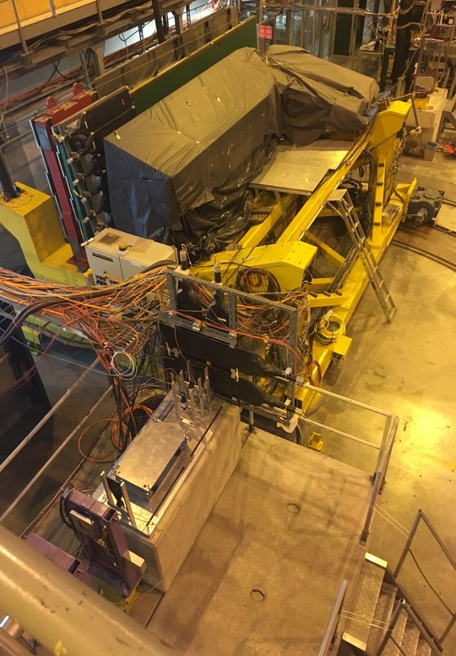
\includegraphics[width=0.6\linewidth]{Figures/Teststand.png}
\caption{The test stand at H2. The scintillator tiles are covered in the black tedlar and the new readout modules are connected in the back. The stand can be shifted so the beam can be aimed at different sections.}
\label{fig:stand}
\end{figure}

Although built to be similar to the HCAL on the CMS detector, the test stand is smaller and has some differences. When looking at the data from the teat beam, it is important to be sure that the e-map, which traces the channels that receive the data to the actual scintillator tiles on the detector, is correct. There are some differences in this map from the test stand and the H2 control room and the HCAL detector and the CMS experiment cavern. In order to account for these differences a new emap was created for the test beam setup. With an accurate e-map we can create an accurate picture of the incident particles hitting the test stand. The test beam allows us to control the energy and type of particles incident on the test stand. This allows us to study things like SiPM non-linearity as we can look at the output of the SiPMs under something like $50 \GeV$ pions then increase to energy to something like $150 \GeV$ and compare the different responses. However the particle does not deposit its energy in a single scintillator tile. For something like a pion, it will lose a part of its energy with each scintillator tile it hits and eventually be stopped by the detector, but its total energy will be spread throughout the detector. Since each particle in the beam has roughly the same energy and we can isolate the event of a single particle hitting the detector we are to find energy lost in each scintillator tile but looking at the complete picture of the detector. 

SiPM non-linearity is not the only thing that is being researched using the test beam. In the CMS detector, particles come so fast that the signals of individual particles blend together. In the test beam, the particles are more spread out so it is easier to isolate the signal of individual particles. This makes it easier to extract the pulse shape of the readout modules which is the shape of the output charge vs. time. It is also important to see if the pulse shape changes significantly under different circumstances such as higher or lower energies. Using the pulse shape of the readout modules we can then extract the individual signals in the CMS detector.

\section{Test Beam Analysis}

With a proper e-map, we can get a picture of the incident particle, observe its path, and see where it deposited its energy. Since the particle does not deposit all of its energy in a single scintillator tile, this is critical when trying to recreate the particle energy. It is also important that there are often a variable amount of scintillator tiles in a single depth channel as shown in figure~\ref{fig:emap} which shows 4 scintillator tiles in depth 5 and 3 scintillator tiles in depth 4. Looking at the results in the plot to the left, it explains why there is more energy deposited in depth 5 rather than depth 4. 

\begin{figure}
\centering
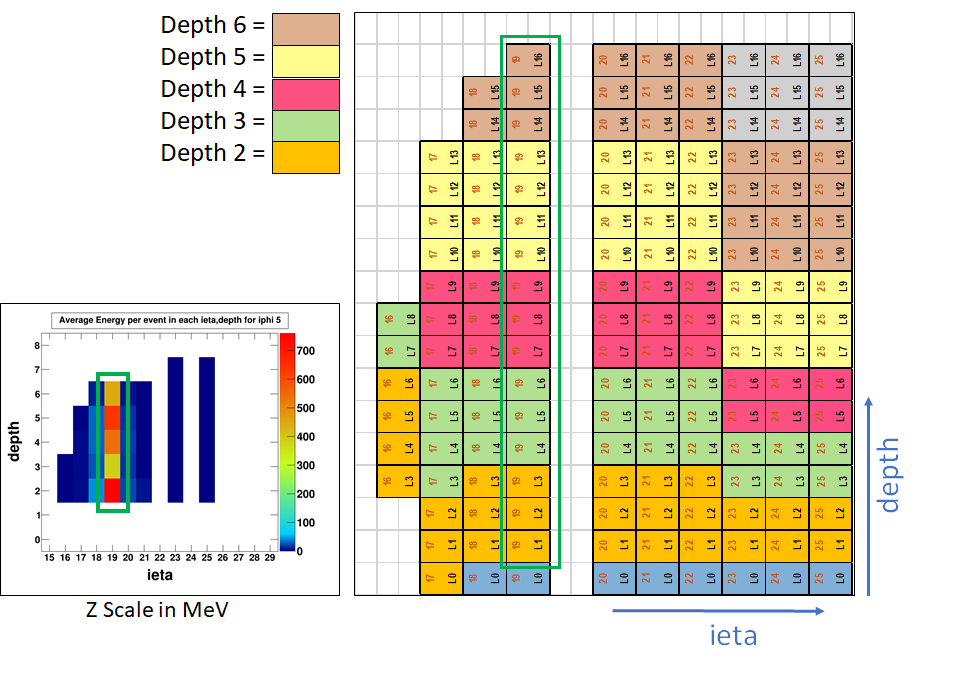
\includegraphics[width=\linewidth]{Figures/eplot.png}
\caption{The emap for a iphi slice of the test stand on the right which was used to create the figure on the left showing the different places the 150\GeV\space muons hit the test stand.}
\label{fig:emap}
\end{figure}

Muons are useful for many things, but when trying to recreate the energy of the particle, it is easier to use pions. The reason for this is that muons tend to go through the detector depositing a small portion of the energy but not being entirely stopped. This can be seen in figure~\ref{fig:emap} which shows the muons depositing a consistent amount of energy in each of the depths even the ones further along in the beam's path. Figure~\ref{fig:Muon} shows that the majority of the events in this muon run produced several hundred femtocoloubms in a single channel of the detector. Trying to recreate the energy of the incident muon would not give the actualy energy, as it would be significantly less than the actual energy of 150\GeV. On the other hand figure~\ref{fig:pionmap} shows a plot with a pion run. This shows that the pions hit the scintillator tiles in depth 2 depositing a large portion of their energy and depositing less and less in the subsequent depths with basically nothing in the last depth. There is also more significant spread compared to the muon run which shows the muons going straight through while the pions leave some energy in the neighboring channels.

\begin{figure}
\centering
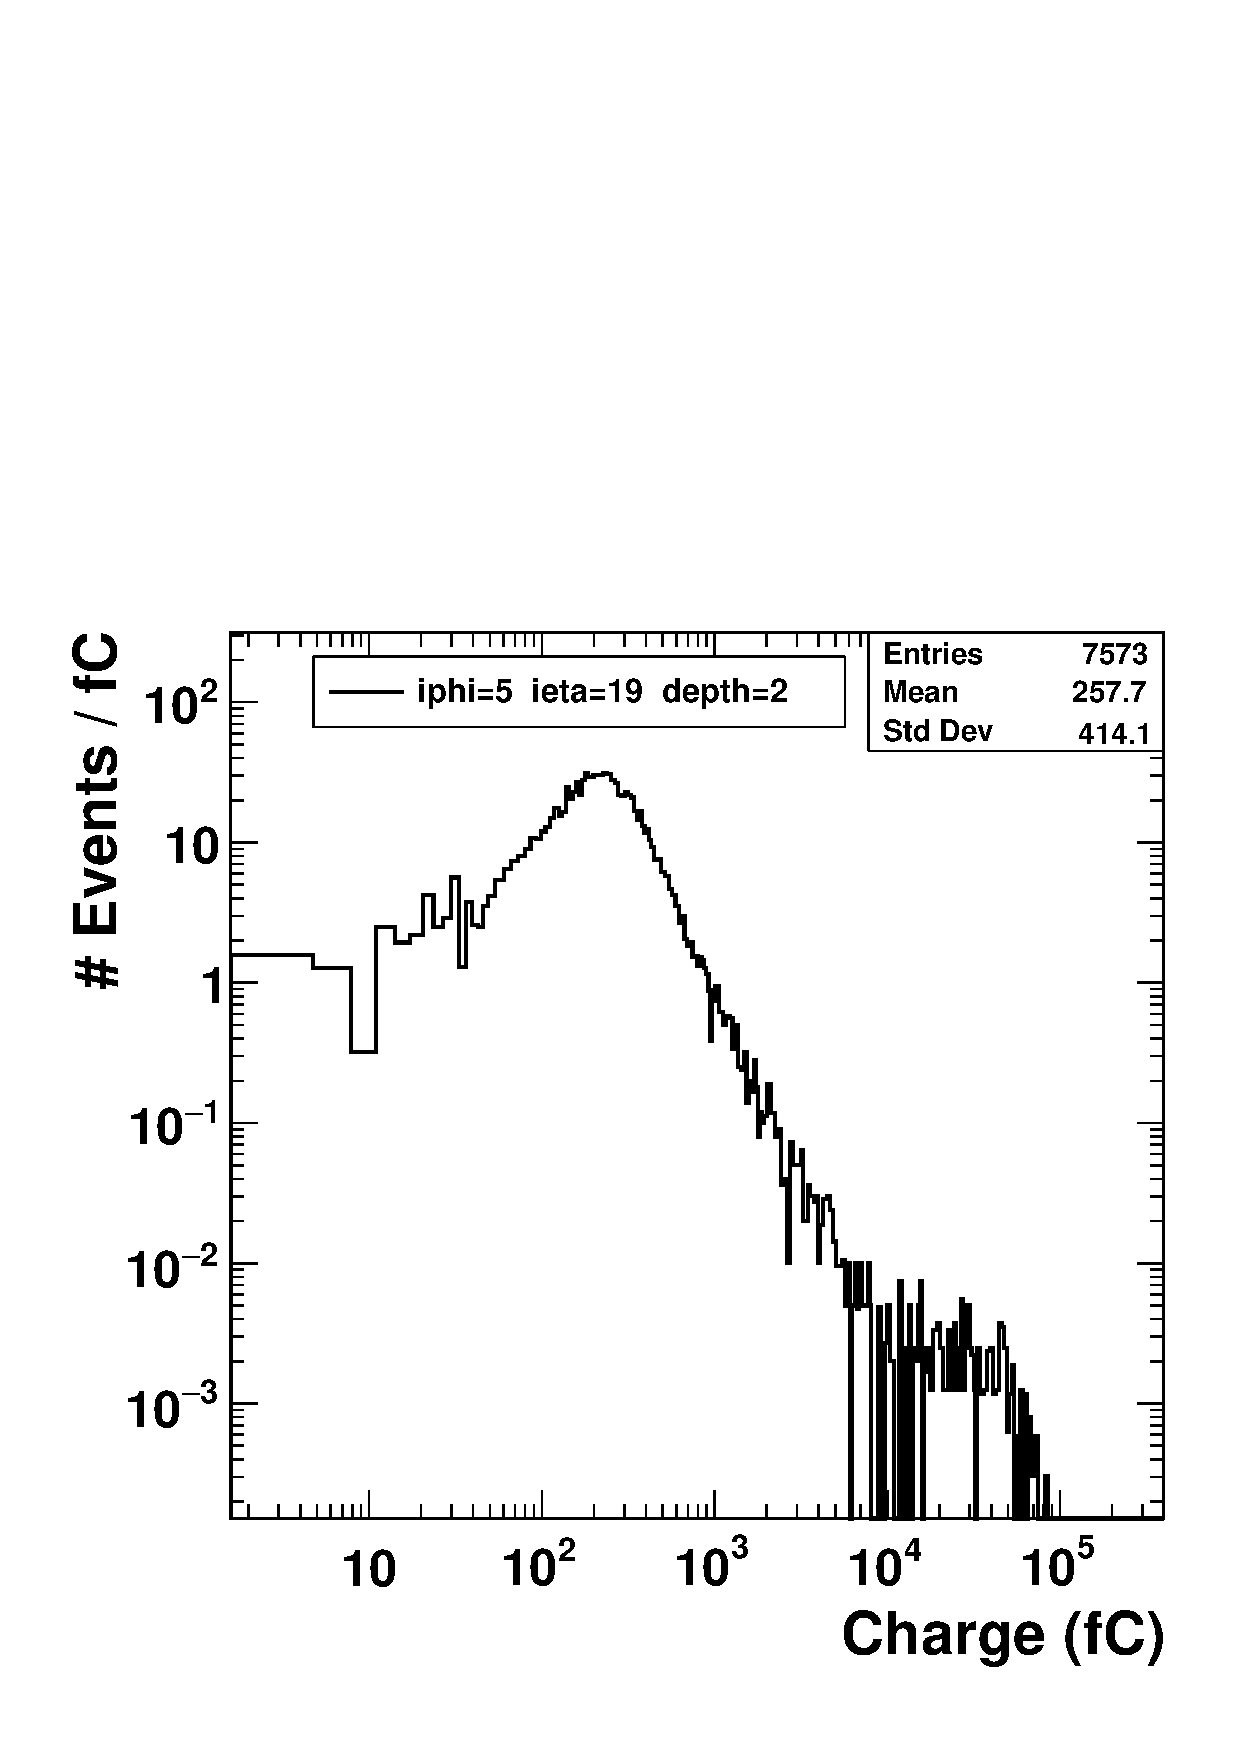
\includegraphics[width=0.7\linewidth]{Figures/MuonCharge.pdf}
\caption{The number of events that output a charge in a channel in a run of 150\GeV\space muons.}
\label{fig:Muon}
\end{figure}

\begin{figure}
\centering
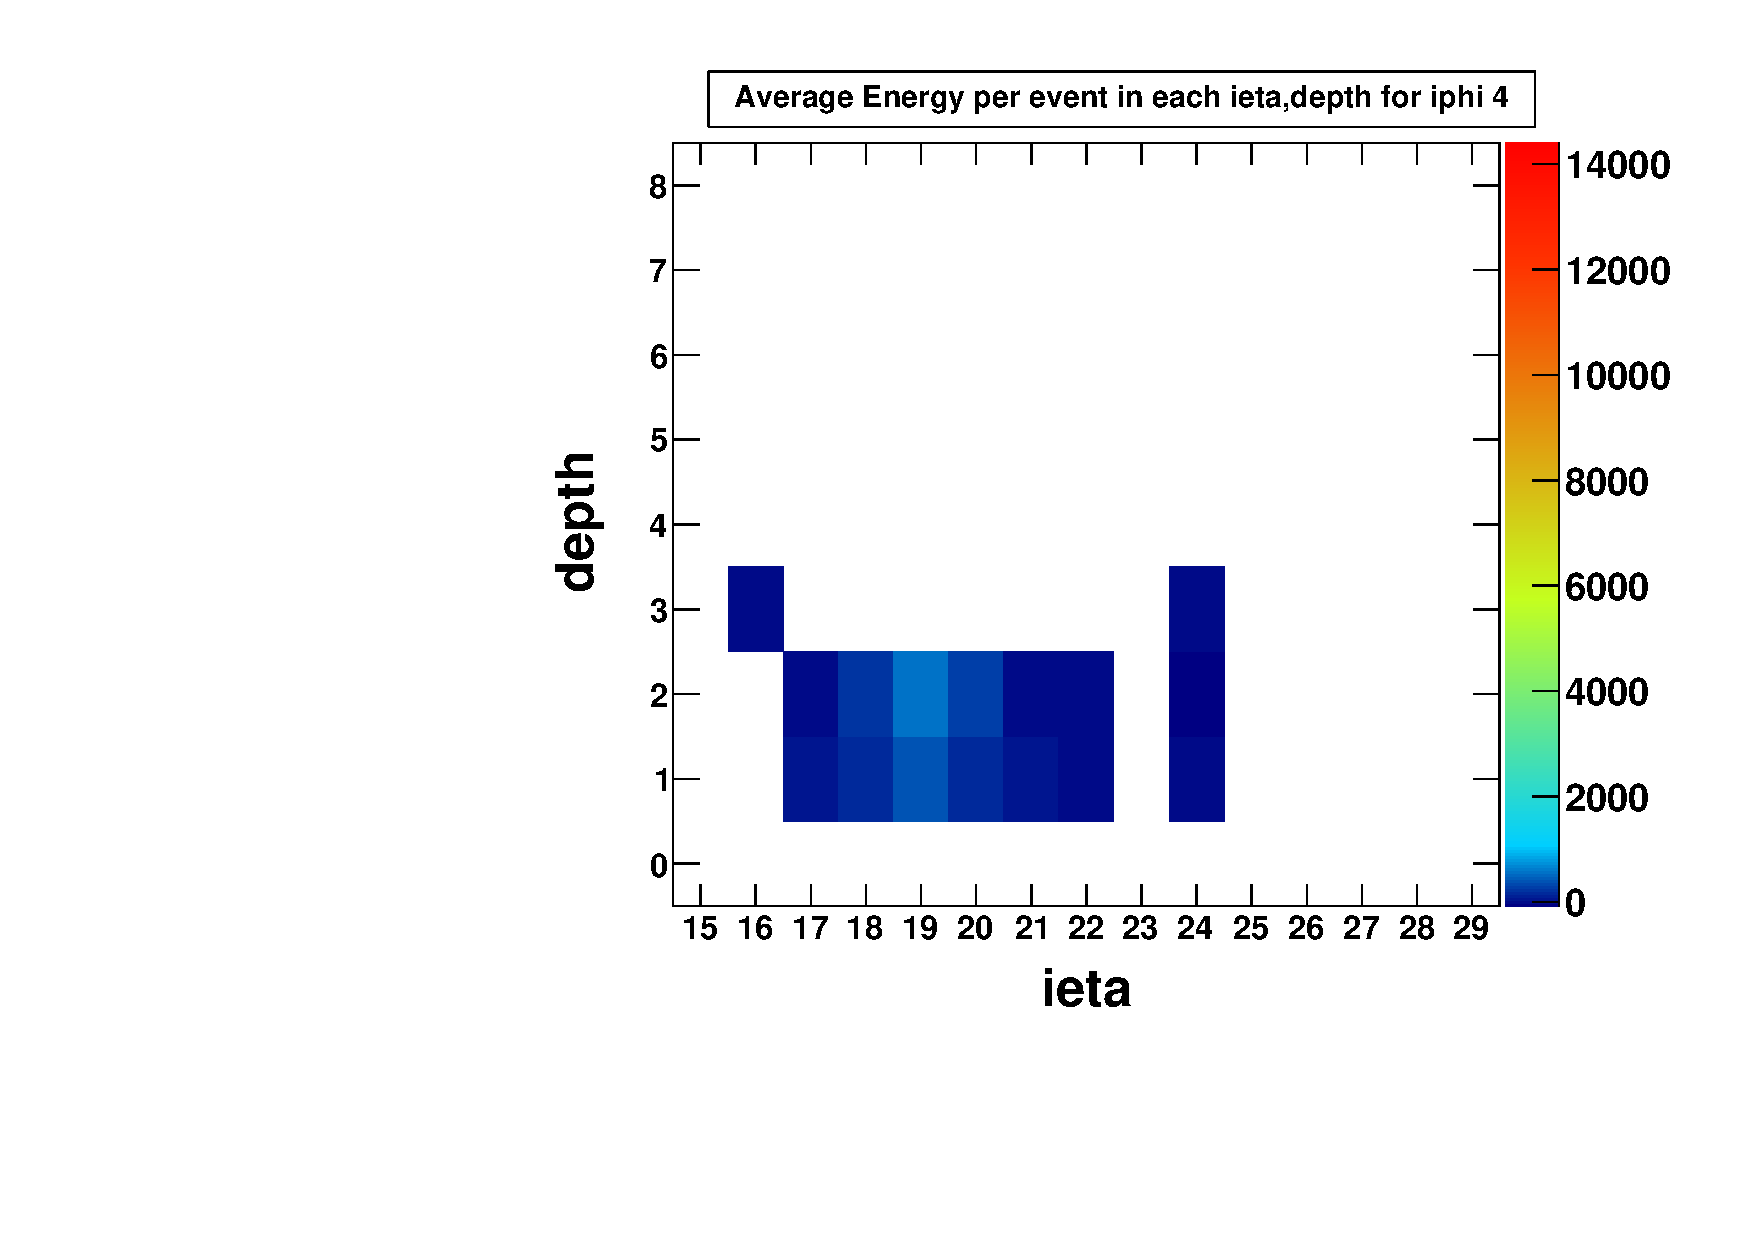
\includegraphics[width=0.495\linewidth]{Figures/pionrun1.pdf}
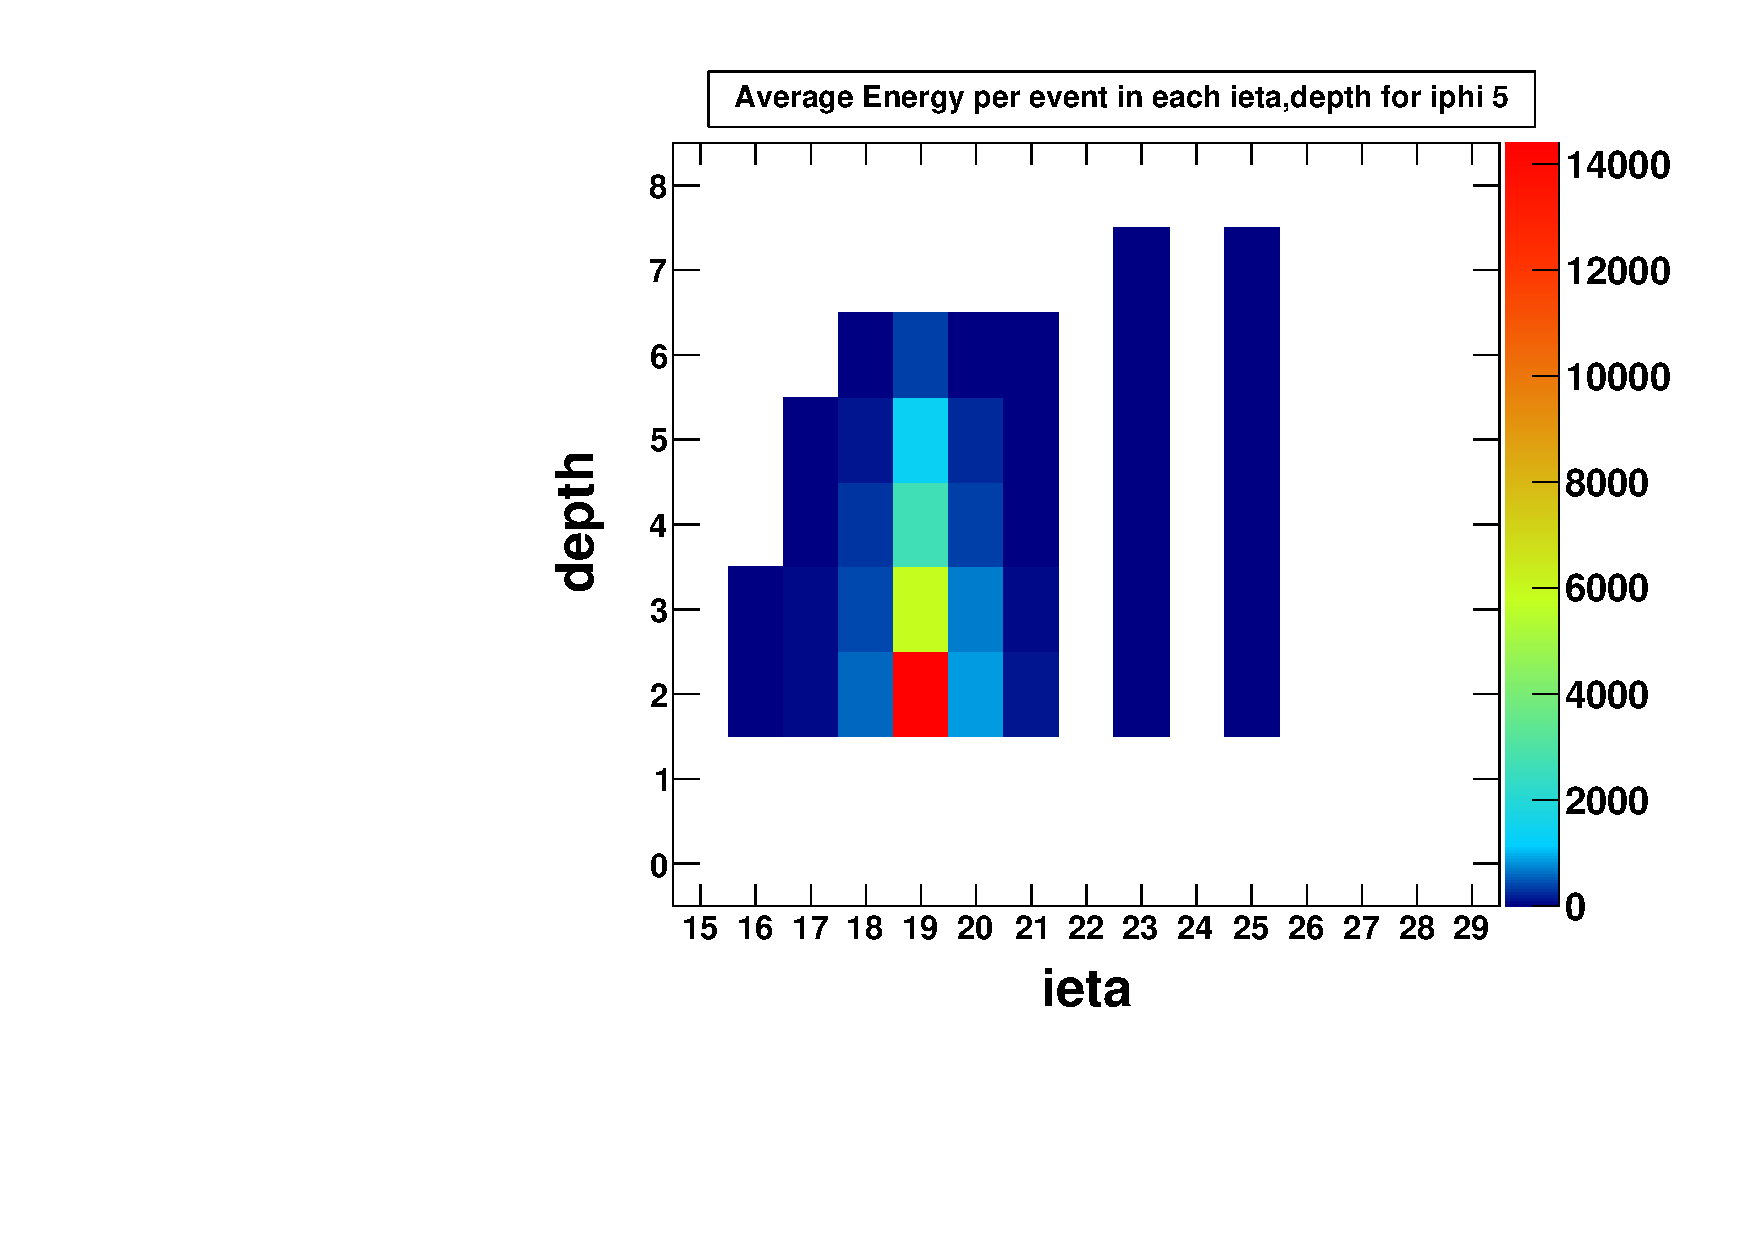
\includegraphics[width=0.495\linewidth]{Figures/pionrun.pdf}
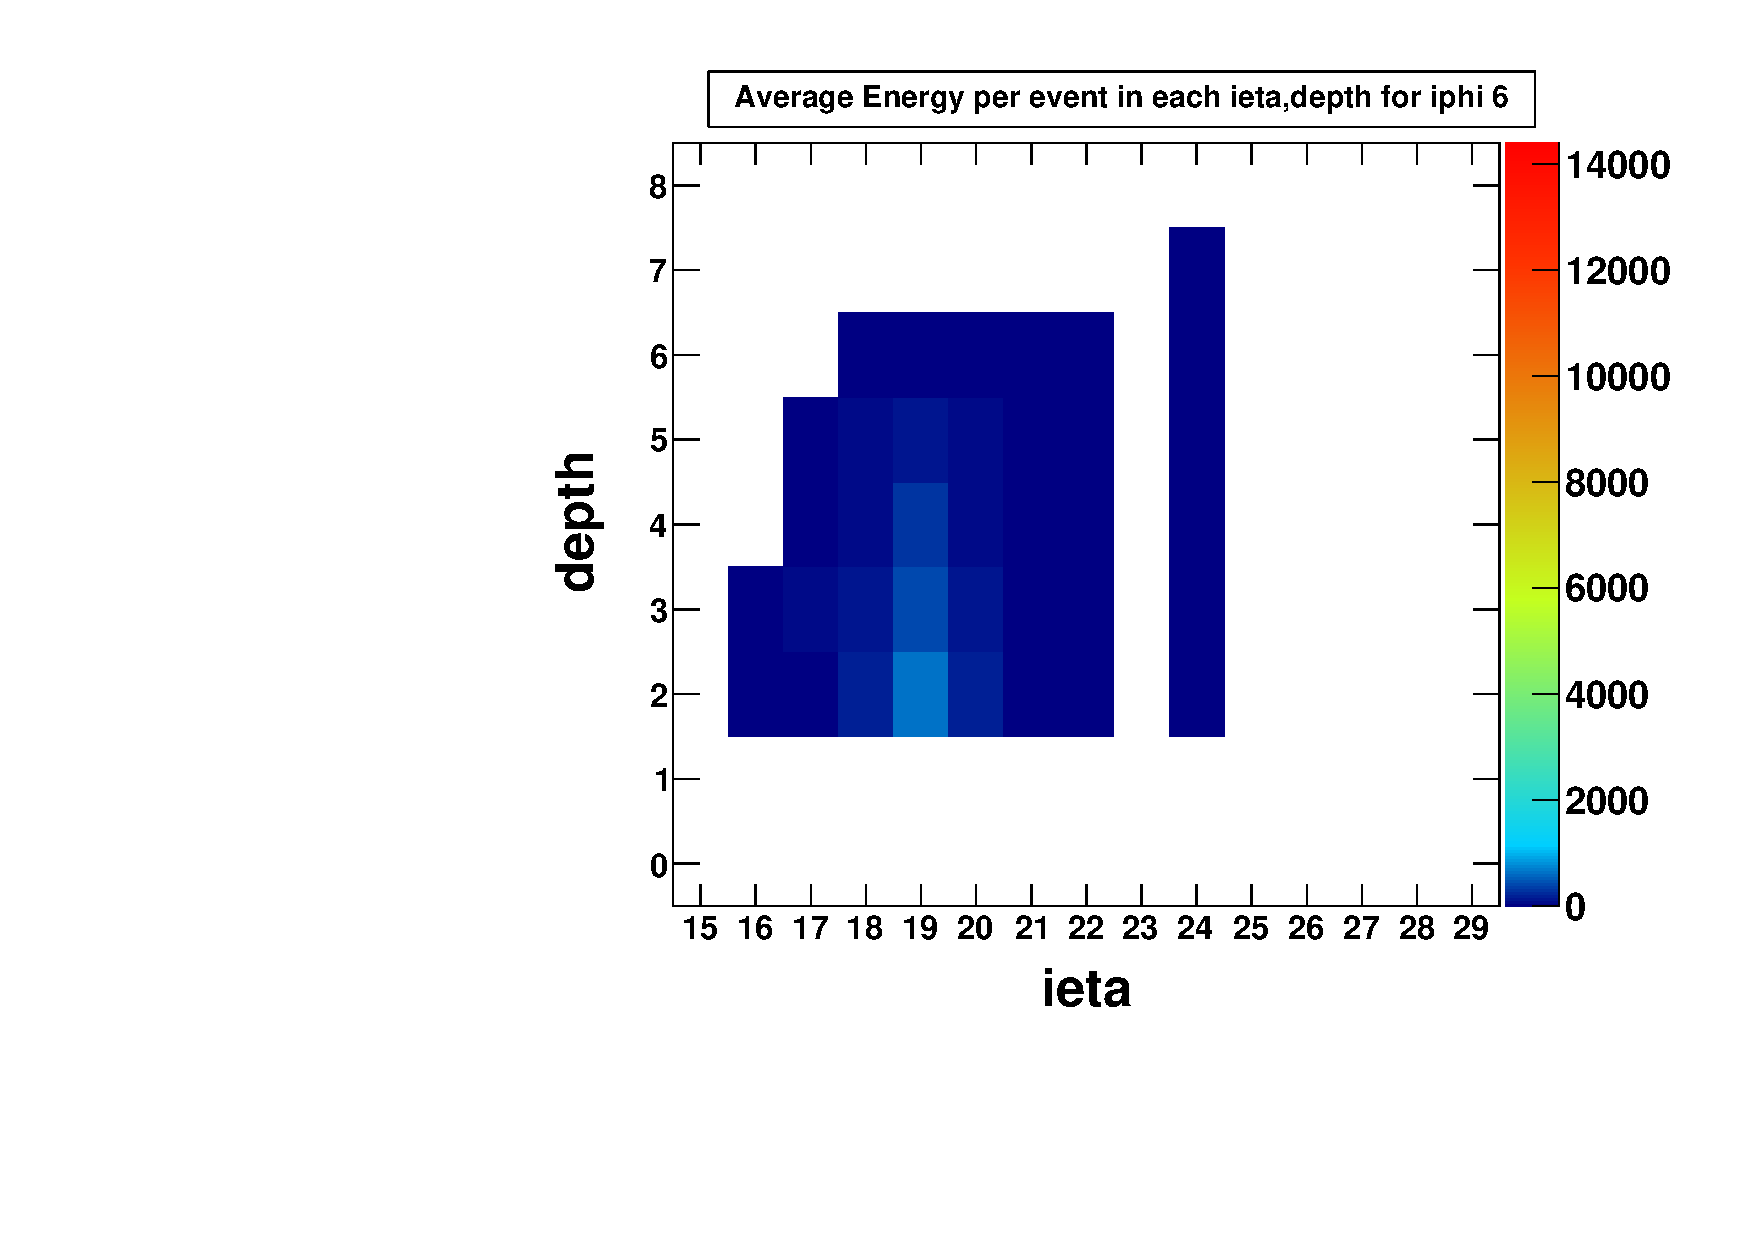
\includegraphics[width=0.495\linewidth]{Figures/pionrun2.pdf}
\caption{A recreation of an event with 50\GeV\space pions showing the pions aimed at iphi 5 ieta 19 and the energy deposited in each channel z scale in \MeV. The different plots show different iphi locations.}
\label{fig:pionmap}
\end{figure}

To recreate the energy of the incident particle we can look at plots such as figure~\ref{fig:pioncharge} which shows the mean output charge in a 50\GeV\space pion run. By looking at this output charge and the output charge of the other channels, we can find what portion of the particles' energy was deposited in this channel and then going by the known energy of the particle how much energy was deposited to produce this output charge. 

\begin{figure}
\centering
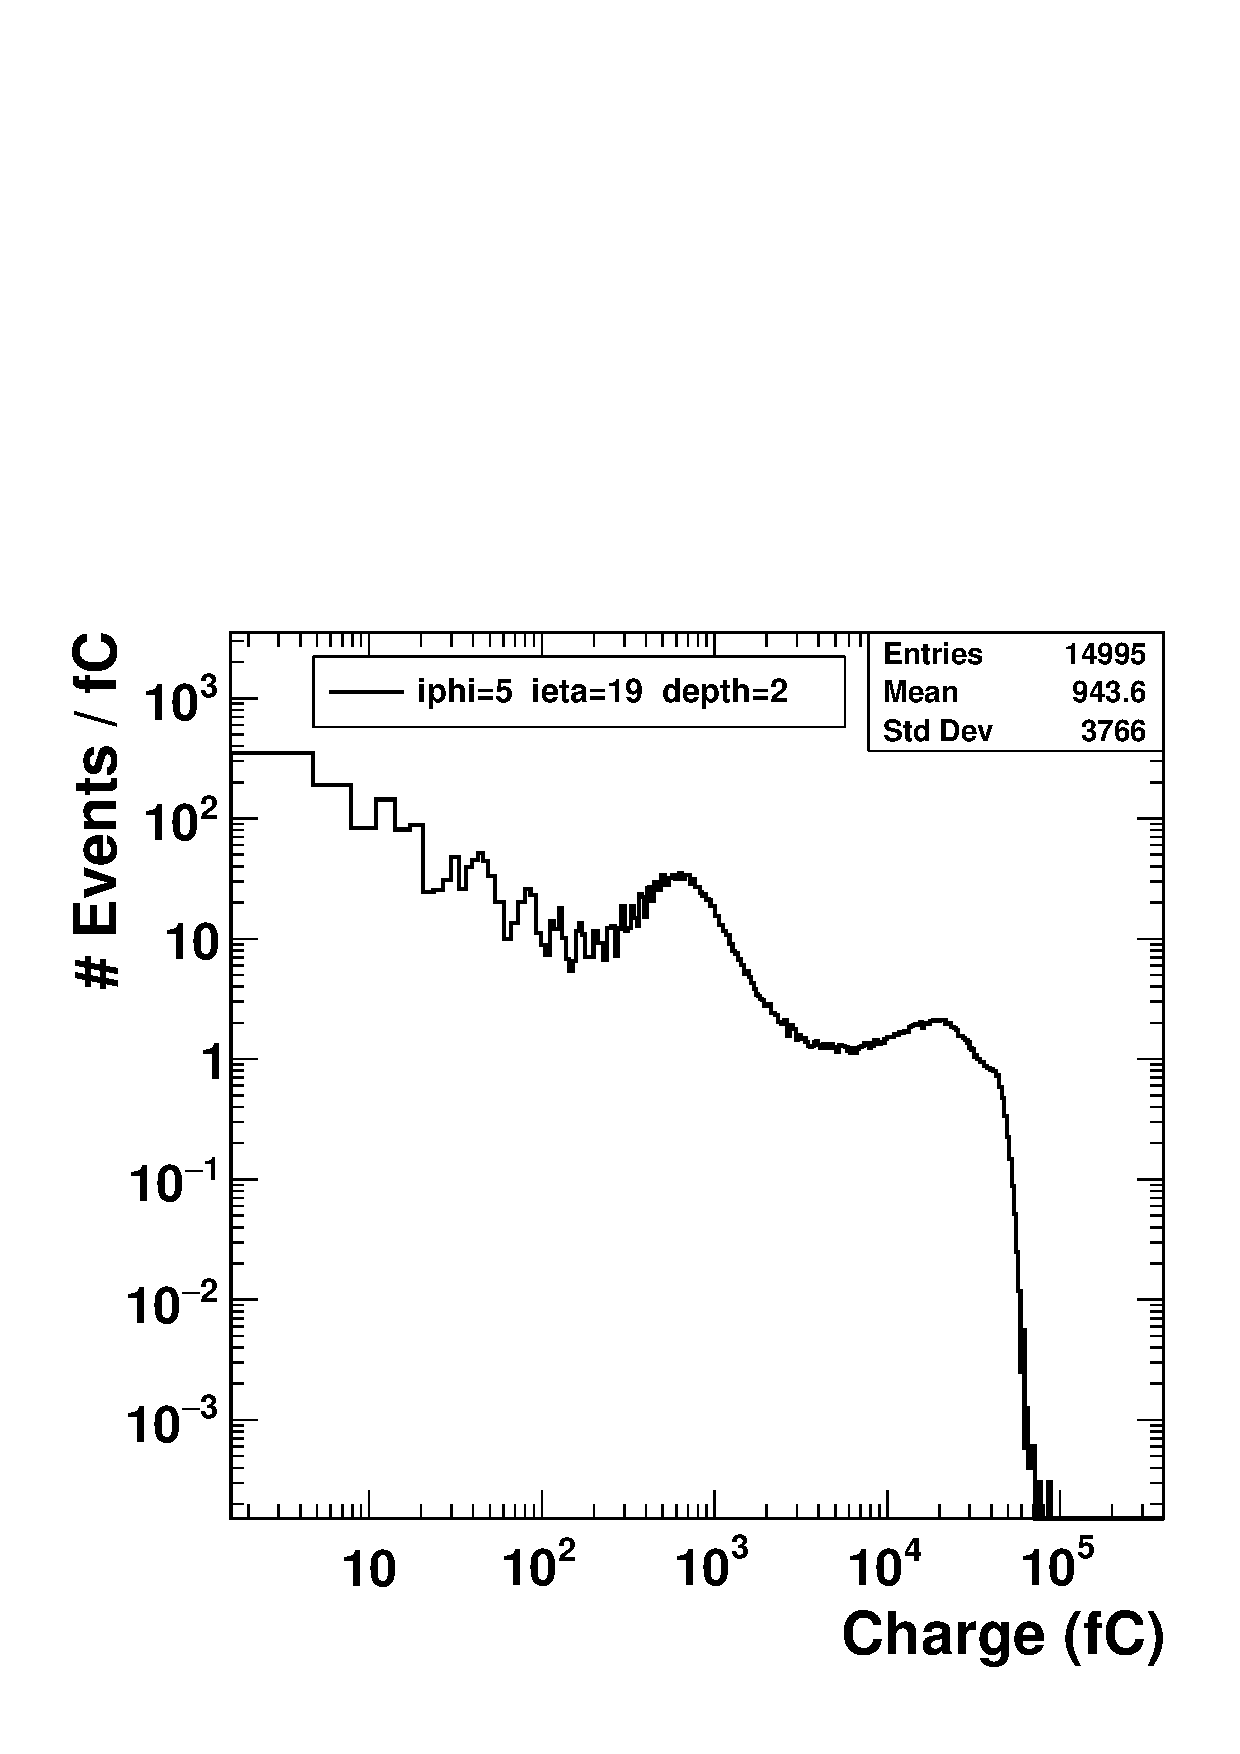
\includegraphics[width=0.7\linewidth]{Figures/pioncharge.pdf}
\caption{The number of events that produces output charge in the SiPM for a run using 50\GeV\space pions. The peak on the right shows the average output charge in response to the incident particles at this energy.}
\label{fig:pioncharge}
\end{figure}

The output charges of the different events can be shown in figure~\ref{fig:Log} which shows the number of events that output a certain charge. This figure can also be used to start the analysis on the SiPM non-linearity. One key thing about the non-linearity is that at low charge output and correspondingly low particle energy the SiPM is very near linear, and it is only at high output charge does this effect become significant. This means to study non-linearity one needs to use particles at sufficiently high energies. After the test beam was over and the analysis of the data was started it was discovered that the test beam was not really capable of producing particles at energies in the non-linear range of the SiPM. To illustrate this looking at figure~\ref{fig:Log} it is apparent that in the $300\GeV$ run, an energy close to the maximum the test beam is capable of producing, there are minimally few events that output charge above 300,000 fC. The SiPM outputs approximately 40 fC for every incident photo electron which means the highest energy events create about 6000 incident photo electrons. When using a simulation of the SiPM it is apparent that this is still very much in the linear range of the SiPM. One thing to note is that not all of a single particle's energy goes to a single SiPM. In figure~\ref{fig:pioncharge} is shows that while the majority of the particle's energy is deposited in the first group of scintillator tiles it hits there is still a signficant portion that is in neighboring channels. Summing over all the channels should give the total energy of the particle but this means that 300,000 fC does not directly translate to $300\GeV$. As the energy of the particle increases its energy will spread out more which means a $600\GeV$ pion will not necessarily deposit 12000 photo electrons in the first channel it hits.

\begin{figure}
\centering
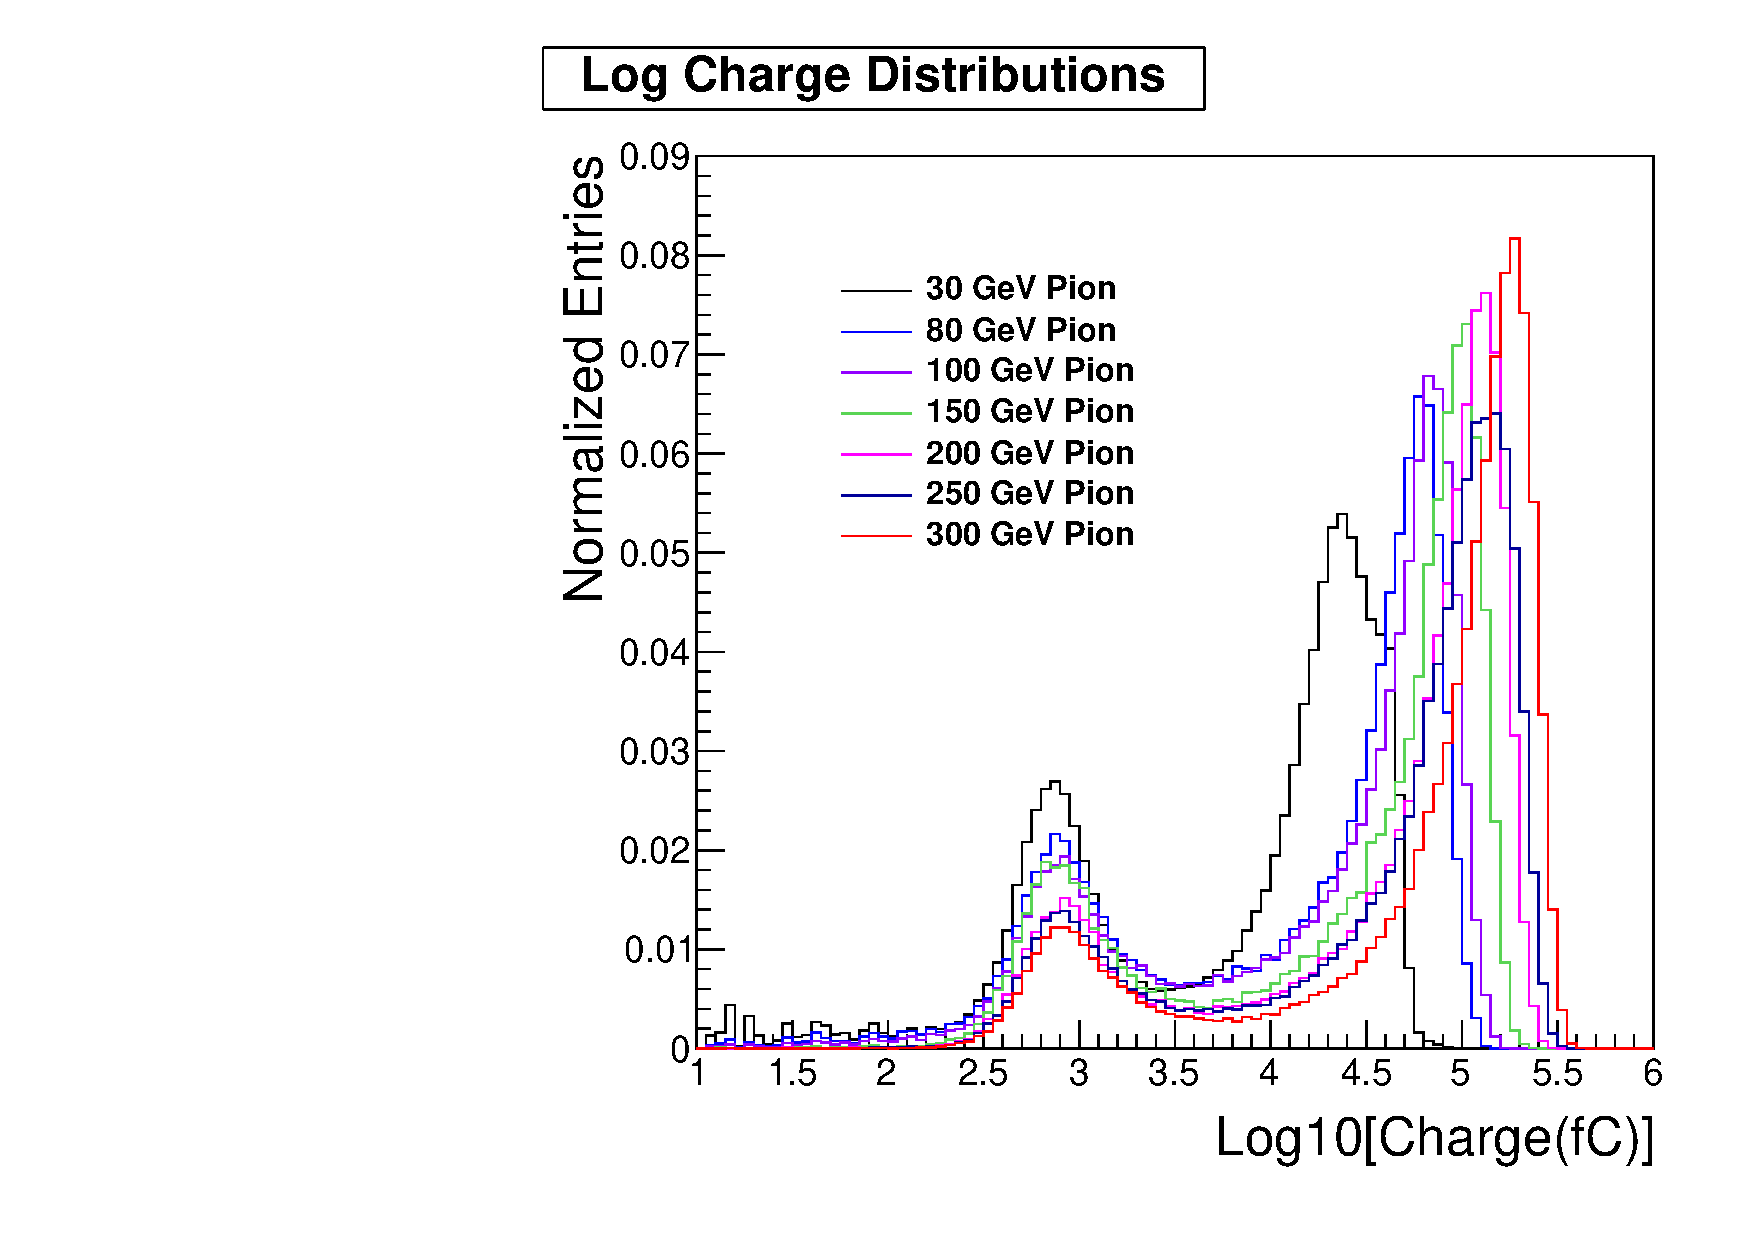
\includegraphics[width=0.7\linewidth]{Figures/Logplot.pdf}
\caption{The charge output of the different events over the different runs used to find the pulse shape.}
\label{fig:Log}
\end{figure}

One of the key things in doing a pulse shape analysis using test beam data is the timing information. In the test beam, we take two different timing information. The first comes from the QIE chips in the readout modules. The readout modules measure the output charge of the SiPM over 250~ns, and the information is binned into 10 time samples each 25~ns long, which is shown in figure~\ref{fig:PulSh}. The output pulse of the SiPM is about 75~ns long, and it usually stays confined to 3 or 4 time samples. In addition we also take what is called a Time to Digital Converter (TDC) value. This value stores at what time in the 250~ns span the output charge of the SiPM crossed a threshold with a 0.5~ns resolution. Since the output charge starts out below this threshold, the TDC value should give the start of the output pulse of the SiPM. For instance, a TDC value of 20 in time sample 4 means the pulse crossed the threshold charge value 10 nanoseconds after the start of time sample 4 or 110 nanoseconds after the start of data taking. One of the problems with the TDC value is that it could be affected by the amplitude of the output pulse as a high amplitude will cross this threshold earlier. To extract the pulse shape we can do something called a phase scan. 

\begin{figure}
\centering
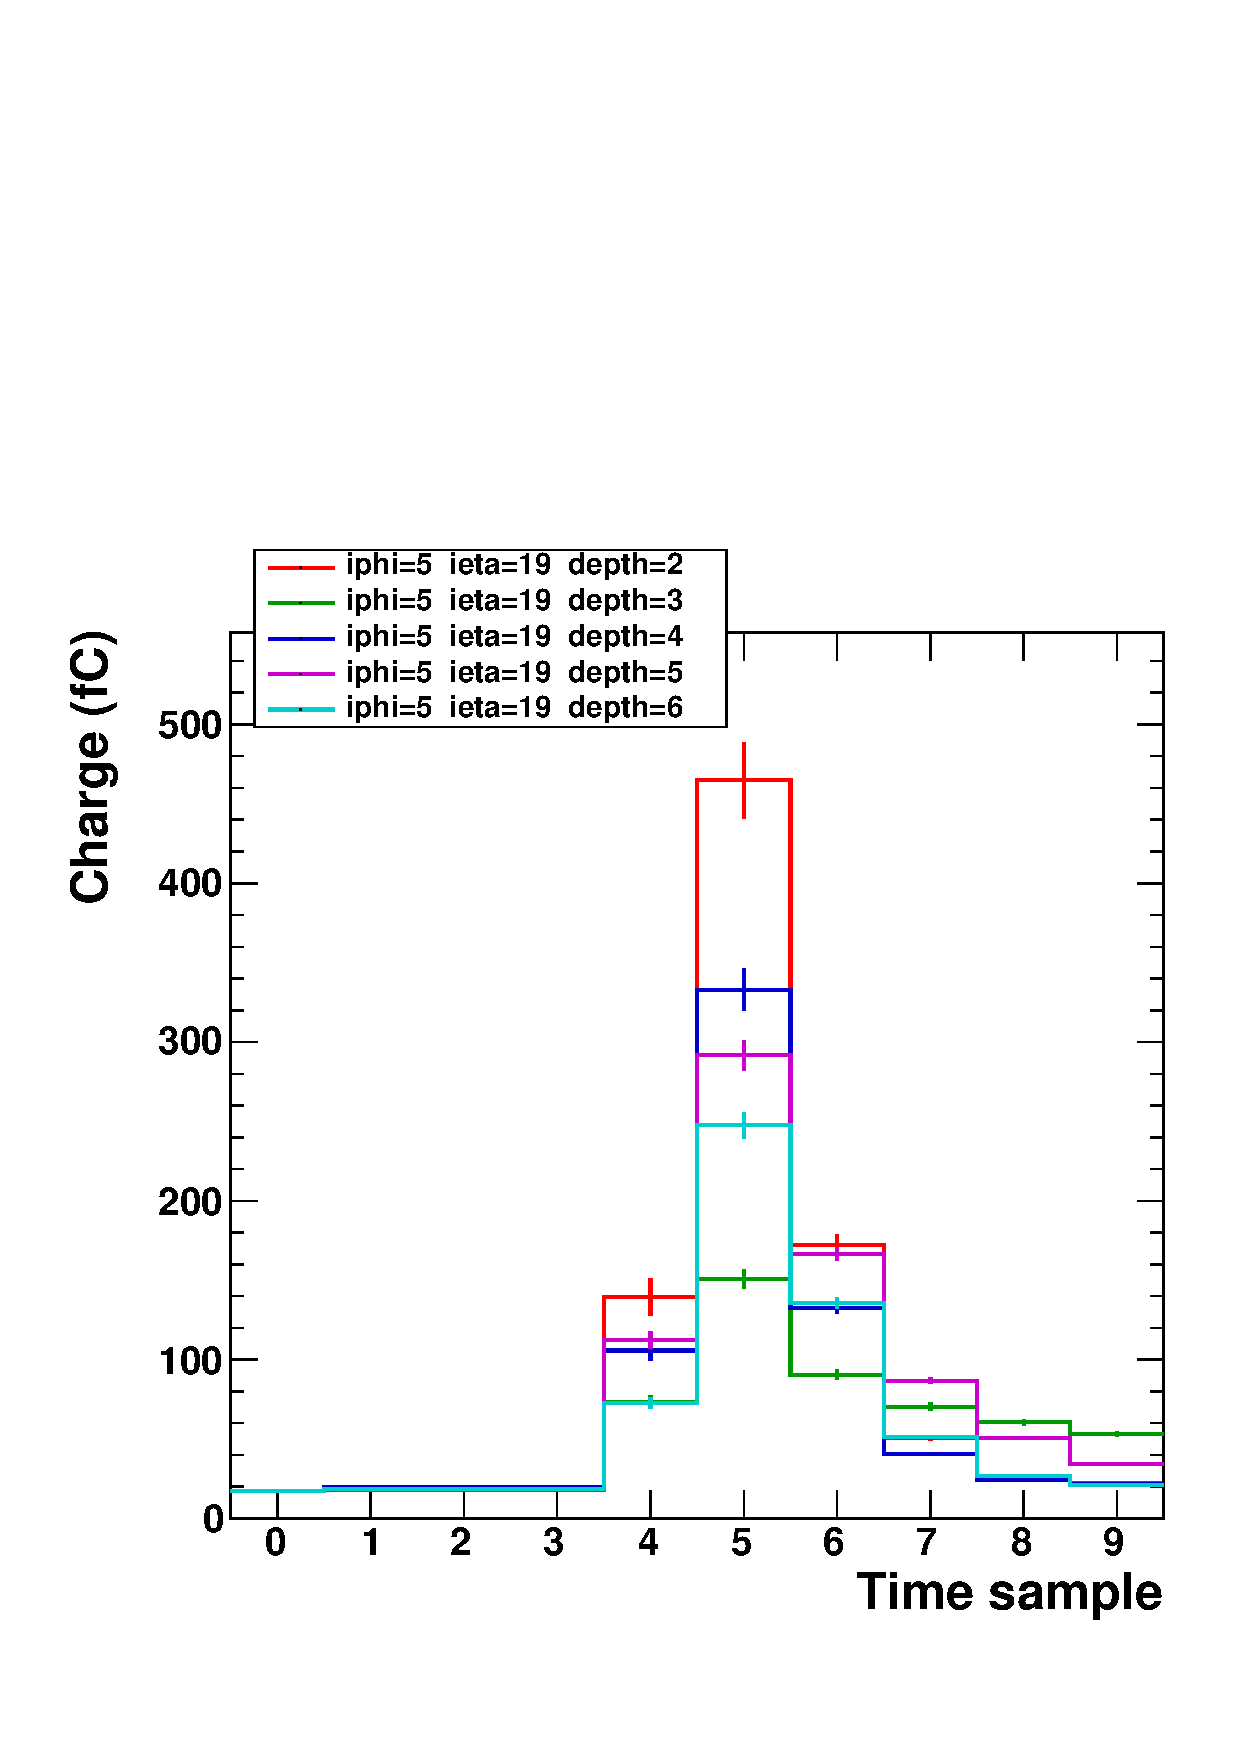
\includegraphics[width=0.6\linewidth]{Figures/Pulse.pdf}
\caption{The output pulse of the readout modules binned in 25~ns bins. This is from a run with 150\GeV\space muons aimed at iphi 5 and ieta 19. This plot shows the output pulse of the different depths at that location.}
\label{fig:PulSh}
\end{figure}

There is also the trigger information. This timing information comes from the test beam equipment that signals the back end electronics to store the data from the readout modules. The trigger information theoretically does not have the same discrepancy as TDC information, but most people still use the TDC from the QIE chips. The relationship between the two signals can be shown in figure~\ref{fig:tdc}. Theoretically this timing information could be used for a phase scan.

\begin{figure}
\centering
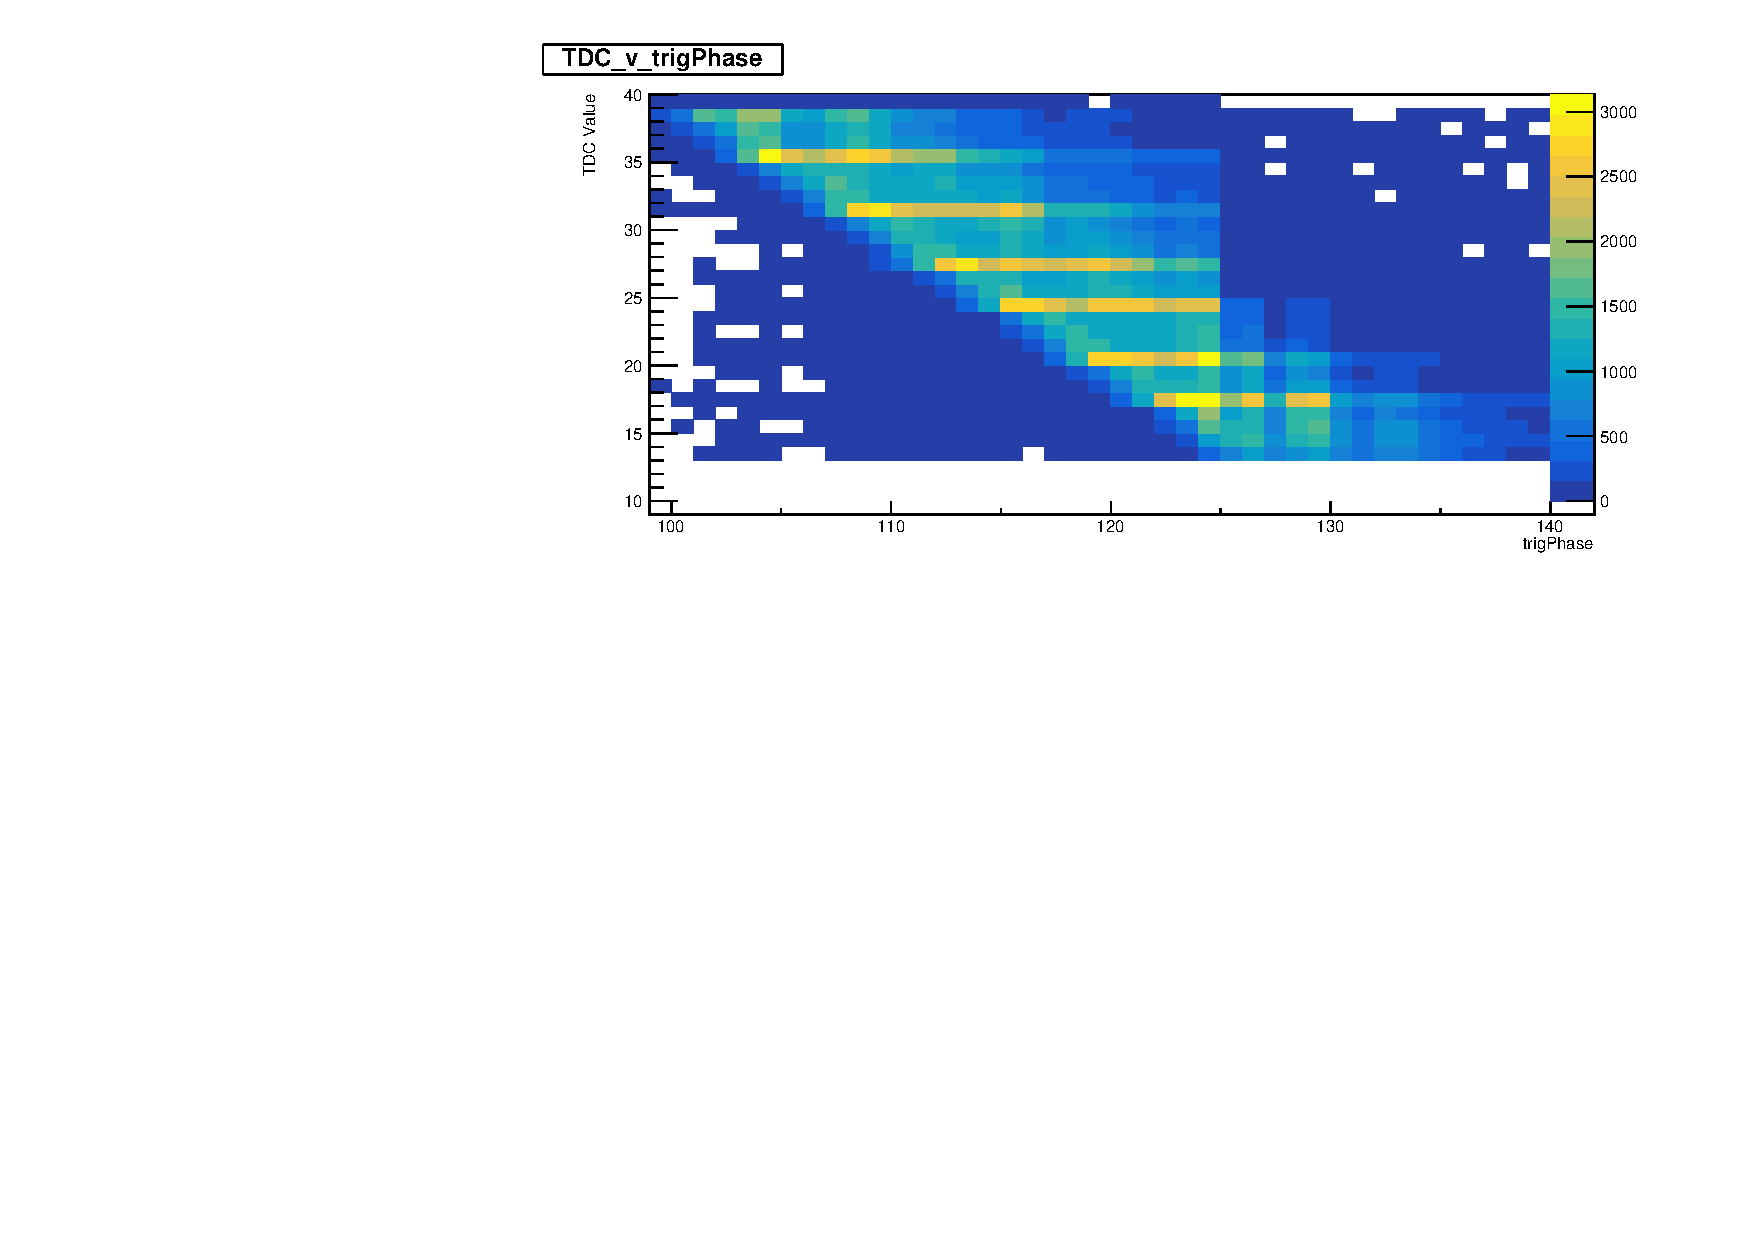
\includegraphics[width=\linewidth]{Figures/TDCvTrigPhase.pdf}
\caption{The statistical relationship between the trigger timing information and the QIE TDC information.}
\label{fig:tdc}
\end{figure}

When we take a run using the test beam, we do not just take data from one single particle but several thousand stored in their own individual events. For instance, when we took a run with $250\GeV$ pions that the run has several thousand events recording the data when the particles all at about $250\GeV$ hit our test stand. Because of the nature of the test beam and also just quantum mechanics there is some randomness to each event. To do a phase scan we take advantage of this randomness by looking at pulses with the same total charge but different TDC values. Theoretically, two pulses with the same charge but different TDC values should be exactly the same except for a time shift. These pulses could look different in data though as different parts of the pulse will be put into different time samples. Figure~\ref{fig:bin} shows an analog pulse shape along with its binned output. A phase scan takes the difference in binned pulse value from several different pulses all with similar overall charge but a range of TDC values. Figure~\ref{fig:Phase} shows multiple sets of data all with different TDC value illustrating how changing the TDC value can change the bins without changing the total output charge. An example of this is taking the difference of the charge value from time sample 4 in a pulse with a TDC value of 20 also in time sample 4 and the charge value from time sample 4 in a pulse with a TDC value of 21 also in time sample 4 gives the pulse height at nanosecond 110 in the 250 nanosecond long data set. Doing this process over all the time samples with more pulses with TDC values ranging from 0-49 all in time sample 4 will give a more analog version of the pulse shape as shown in figure~\ref{fig:fit}.

\begin{figure}
\centering
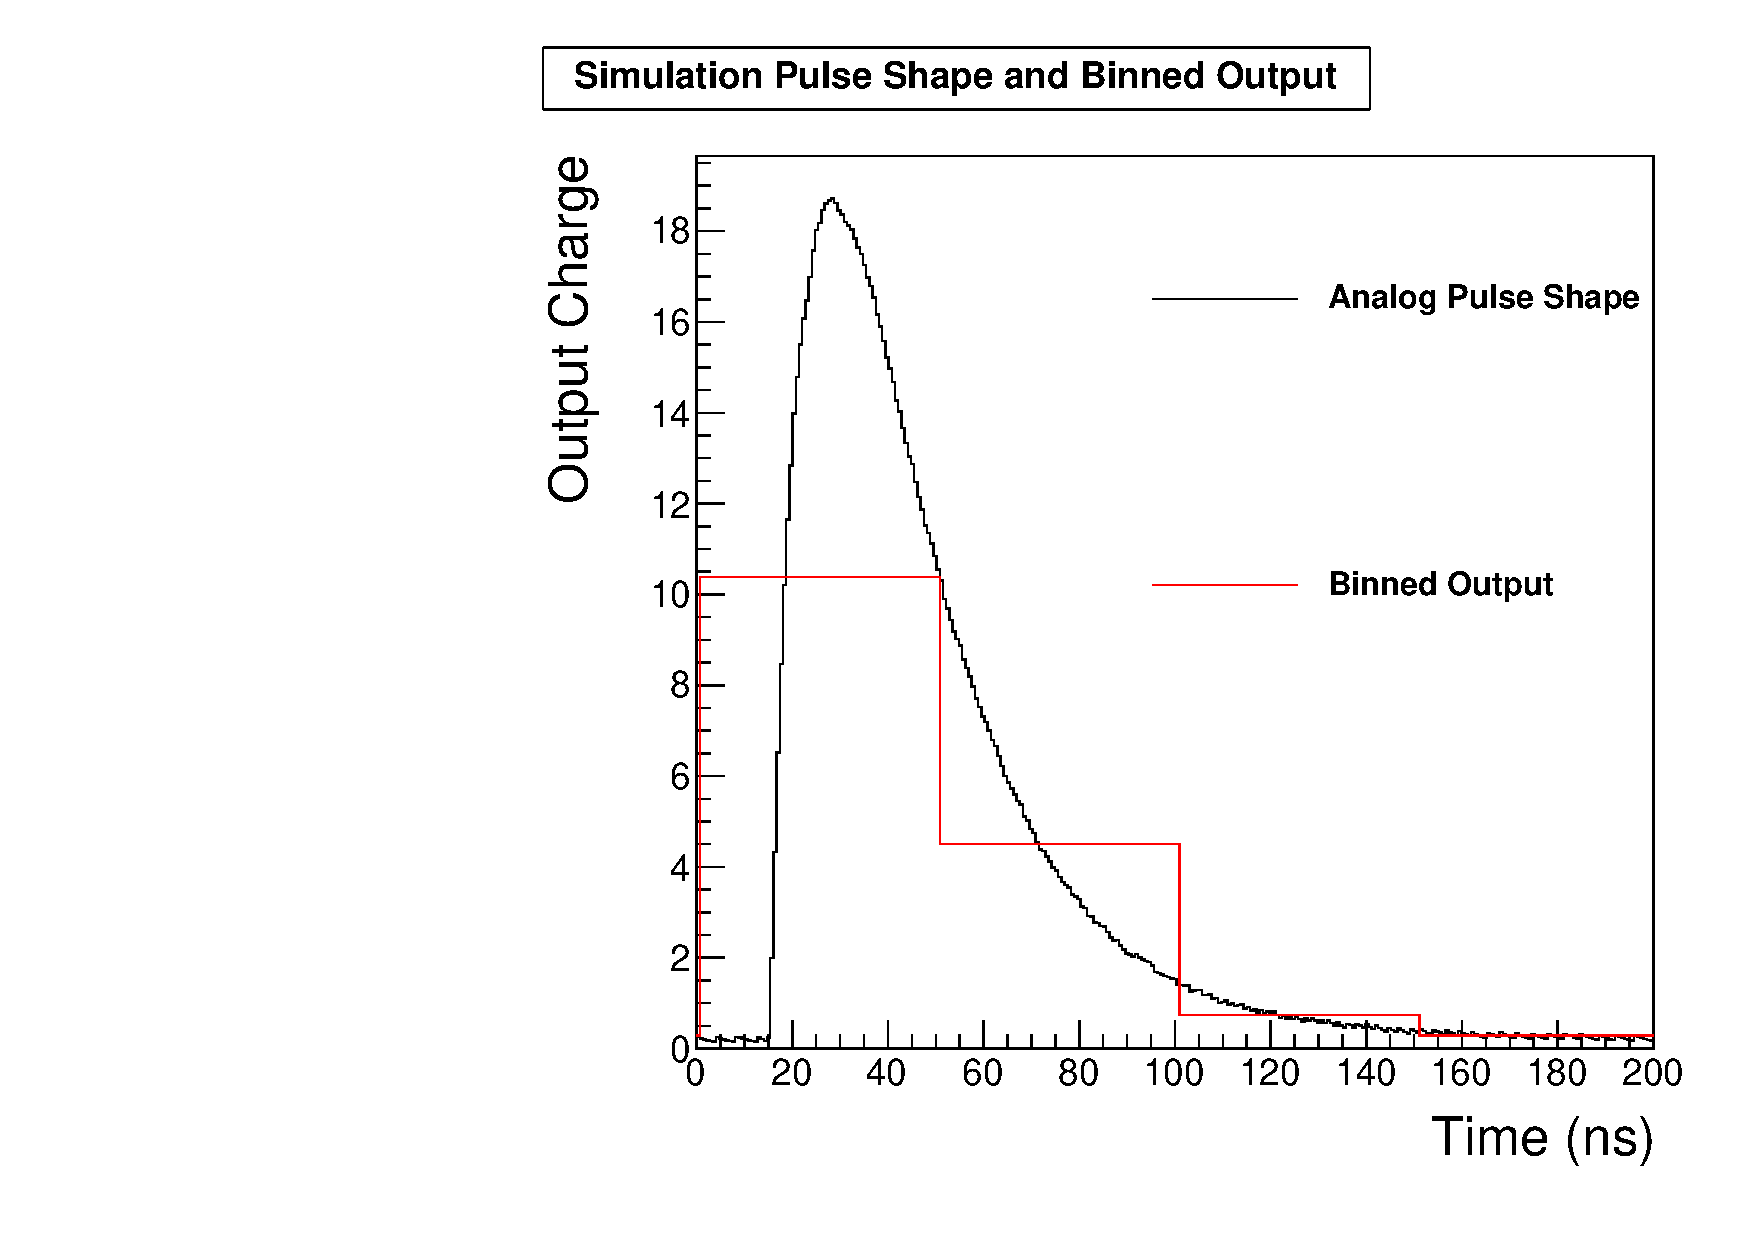
\includegraphics[width=0.6\linewidth]{Figures/Bin.pdf}
\caption{A SiPM simulation showing an analog version of the output charge along with the same output binned in 25~ns bins.}
\label{fig:bin}
\end{figure}

\begin{figure}
\centering
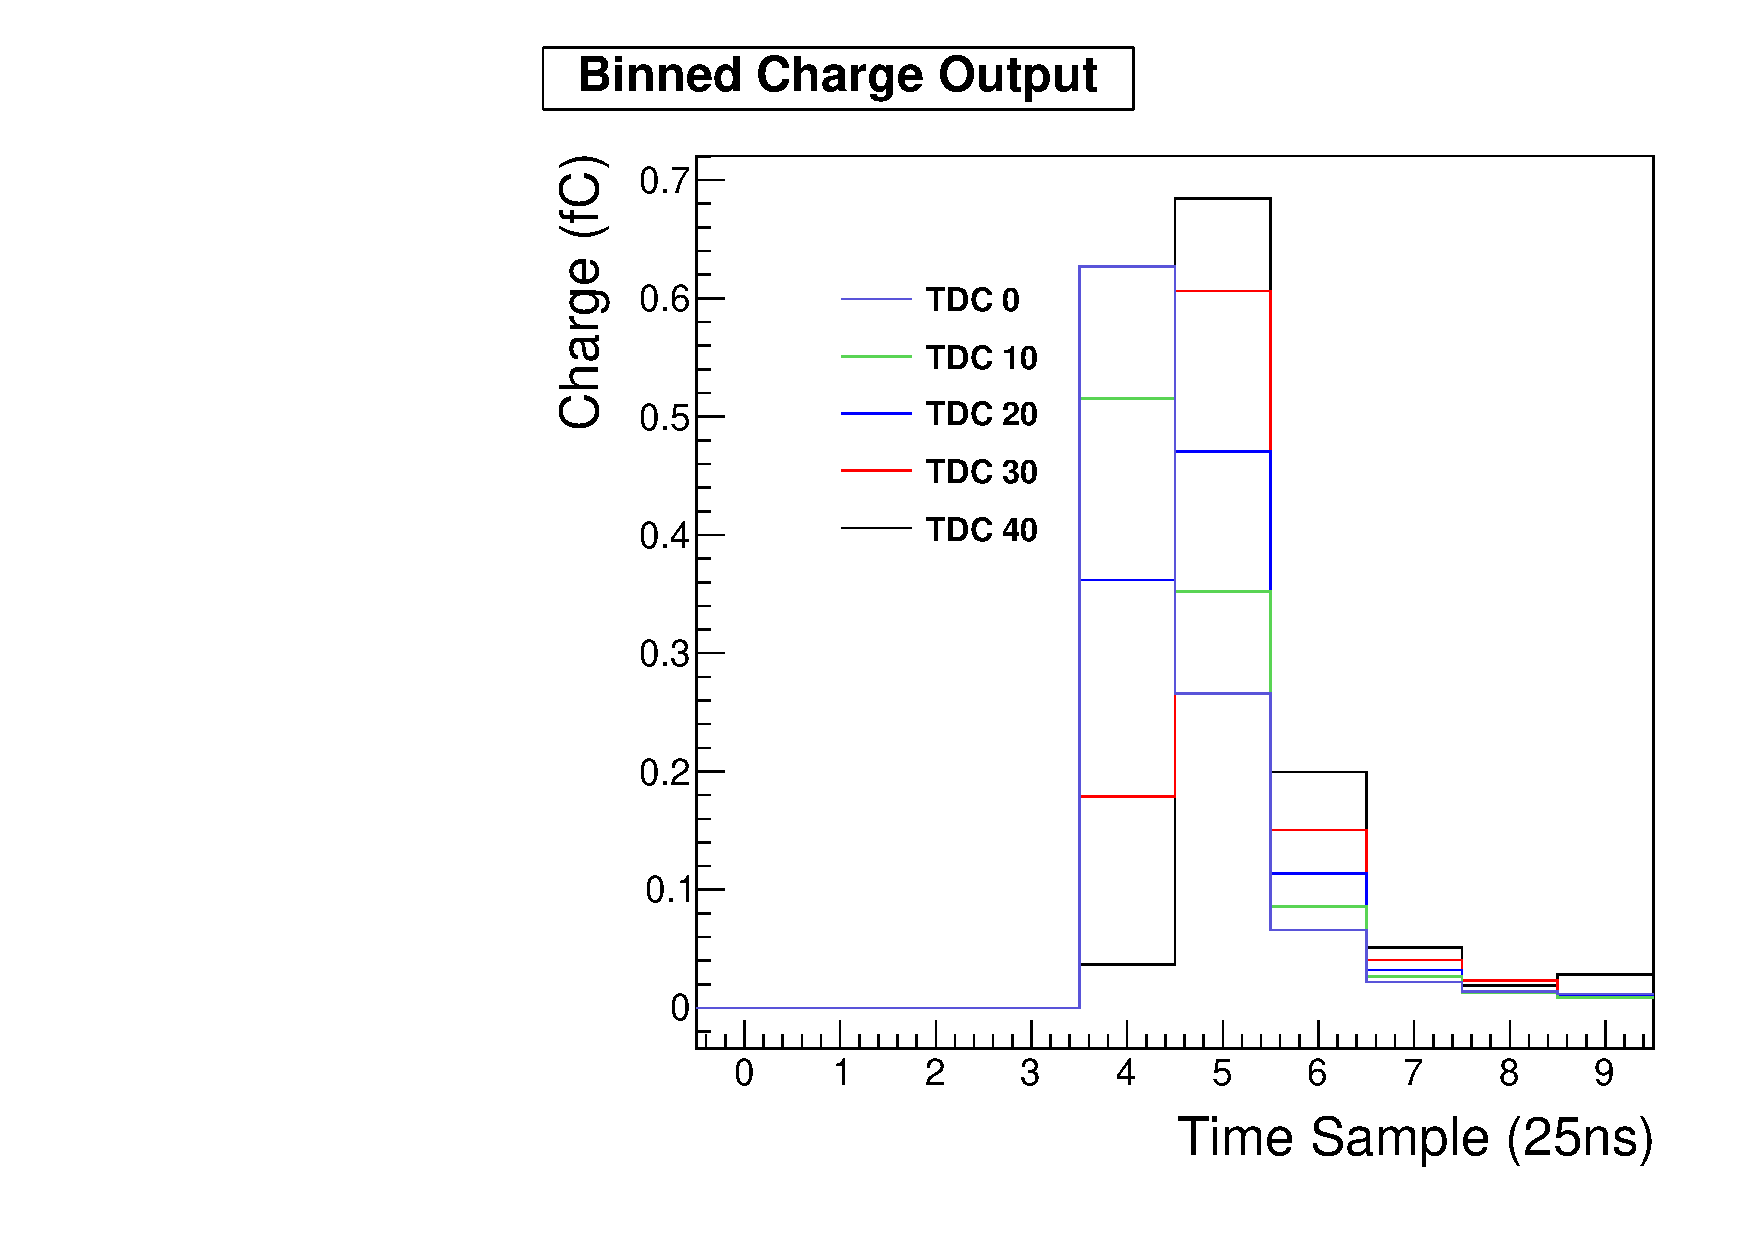
\includegraphics[width=0.6\linewidth]{Figures/Phase.pdf}
\caption{The binned output charge of events with different TDC values. All pulses have their TDC value in time sample 4 and have a total output charge in the range of 50,000-80,000 fC}
\label{fig:Phase}
\end{figure}

\begin{figure}
\centering
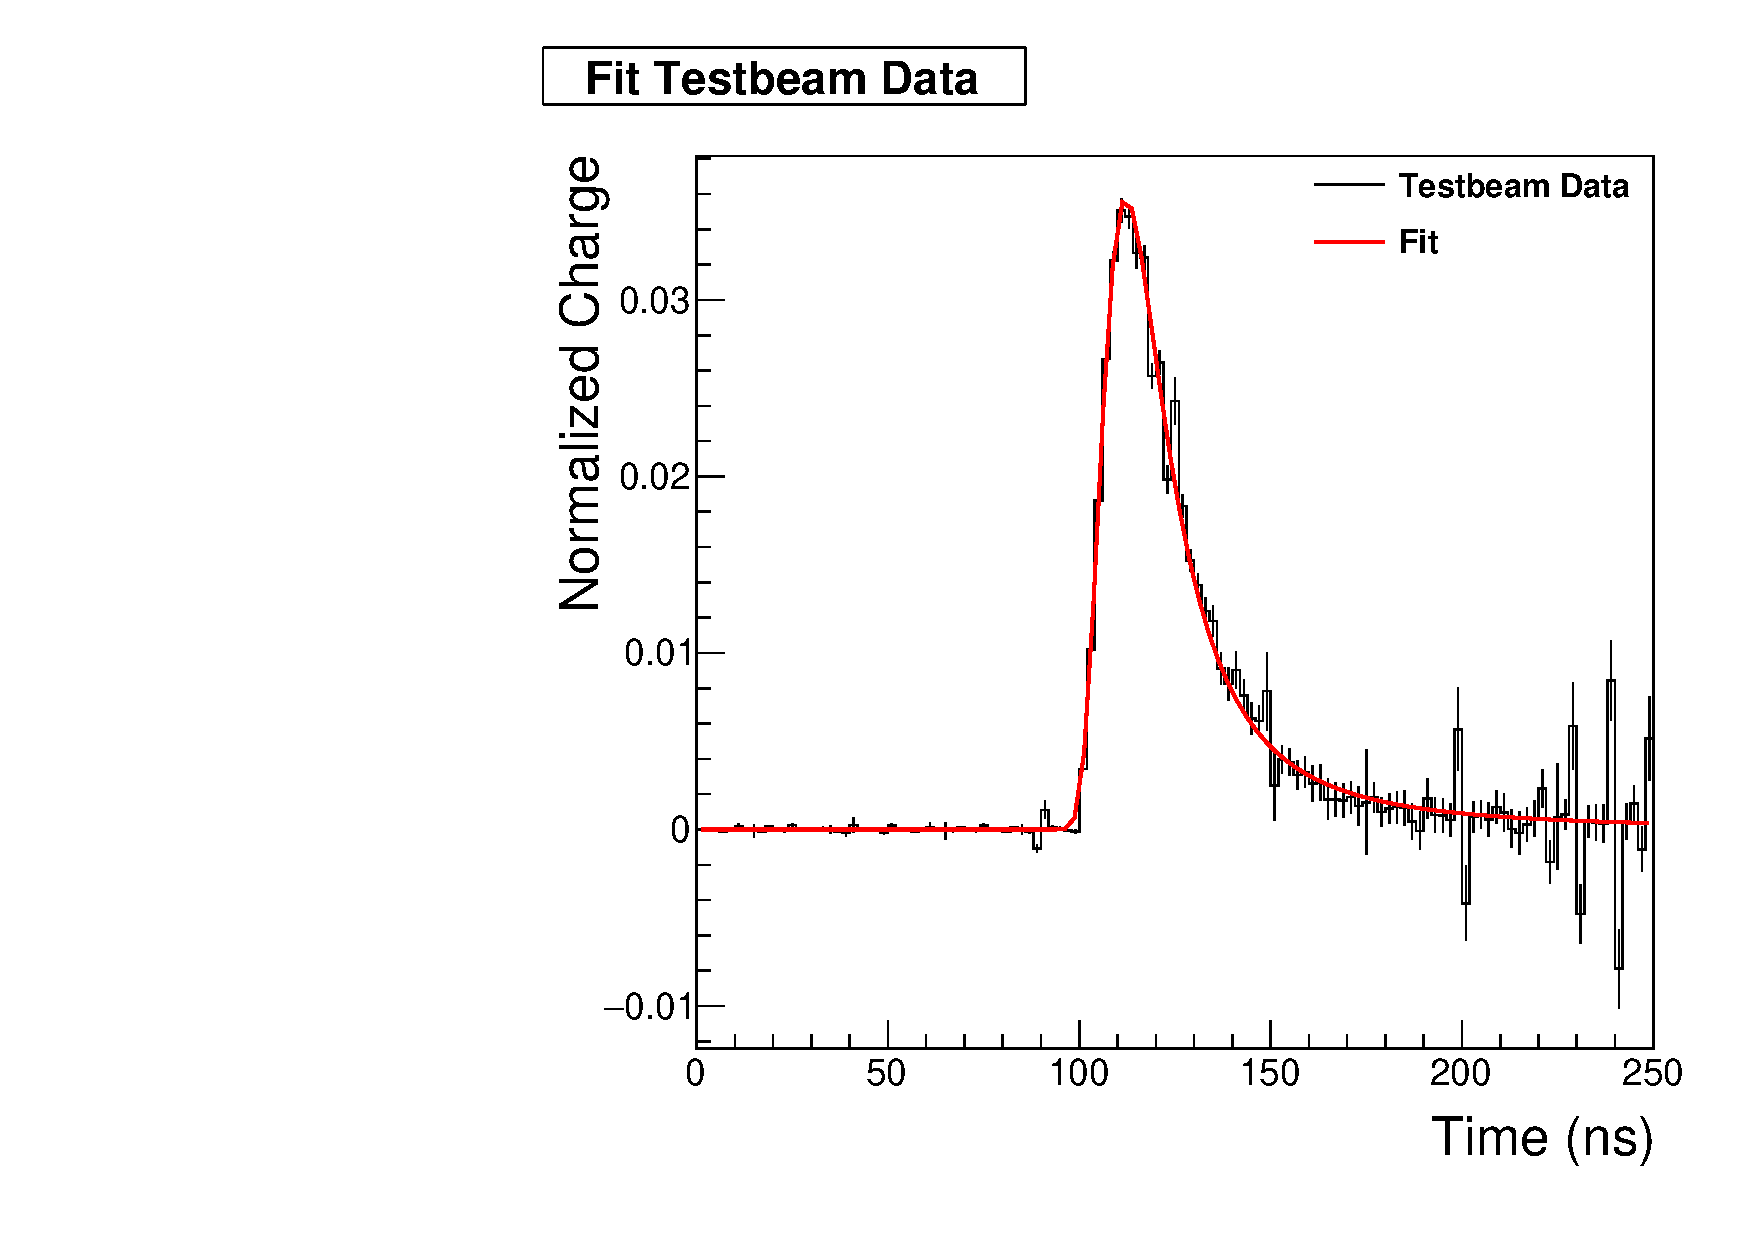
\includegraphics[width=0.6\linewidth]{Figures/FittedPlot.pdf}
\caption{A more analog version of the SiPM pulse shape obtained using a phase scan on test beam data. It is also fitted by a Landau Gaussian function which is what we expected from theory. The total output charge of the runs used in this range from 10,000-29,000 femtocoulombs.}
\label{fig:fit}
\end{figure}


To do a phase scan properly, we need to use events that have similar output charge. There are a variety of reasons for this, but one of them is that there is evidence that the pulse shape may change with output charge. To study this we simply have to do a phase scan using event with different output charge and see if there are any significant changes. Although most of the particles will have the energy set using the beam, it is common to have outliers.. To minimize this disturbance we take in all the events from several different runs energies ranging all the way from $30 \GeV$ to $300 \GeV$ and only use the events that fall within a certain charge range. Figure ~\ref{fig:fit_together} shows pulse shapes obtained using several different charge ranges. Figure~\ref{fig:Overlap} shows the fits of these pulse shapes overlapping for comparison purposes. The fits show that there is little change of the pulse shape as the charge increases but there is a small trend visible in this plot. Looking at the peak of the pulses it is apparent that the lower charge pulses have shorter peaks. This lack of area is made up in the second half of the pulse as the lower charge pulses are slightly higher there though this is harder to see as it is over a longer period of time. This result is not unexpected as the non-linearity of the SiPM can shift the charge of the pulse towards the front. 


\begin{figure}
\centering
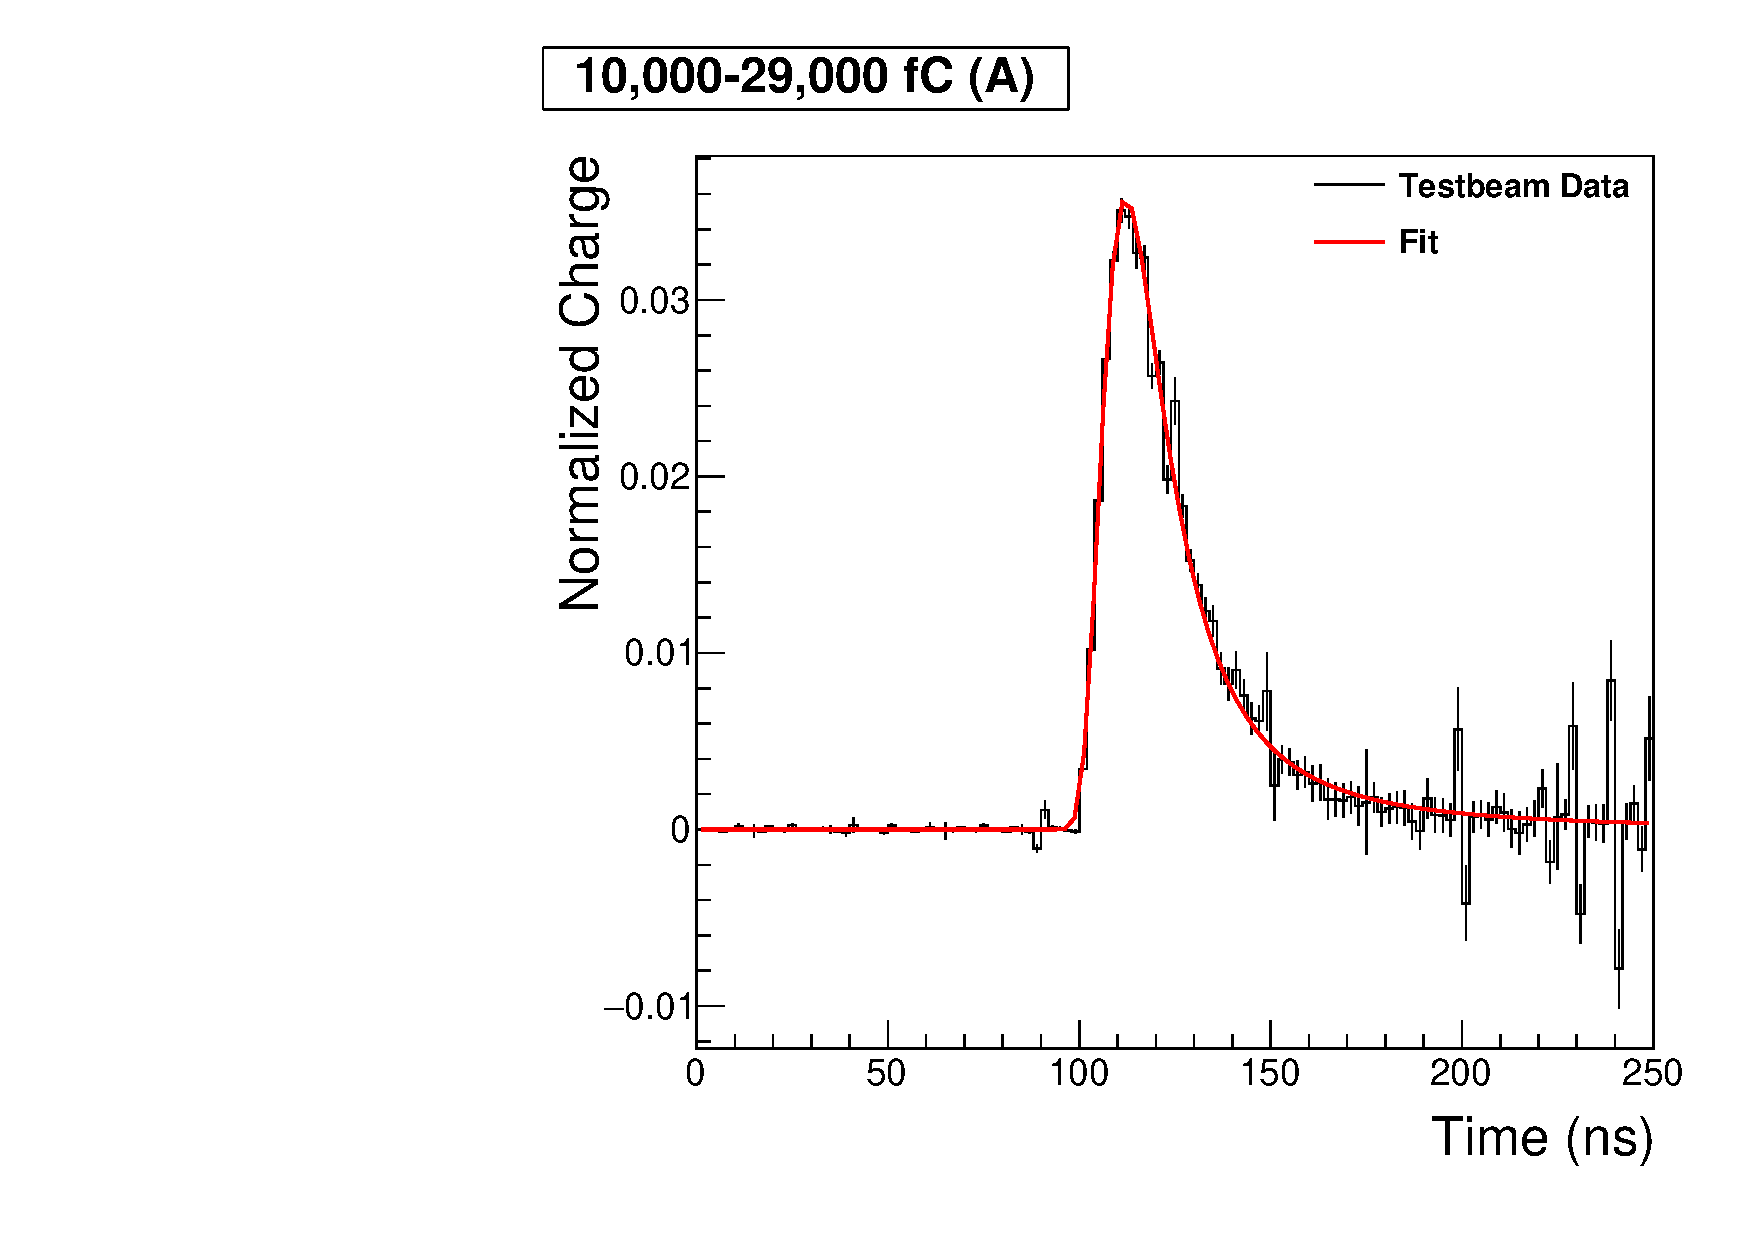
\includegraphics[width=0.495\linewidth]{Figures/10FittedPlot.pdf}
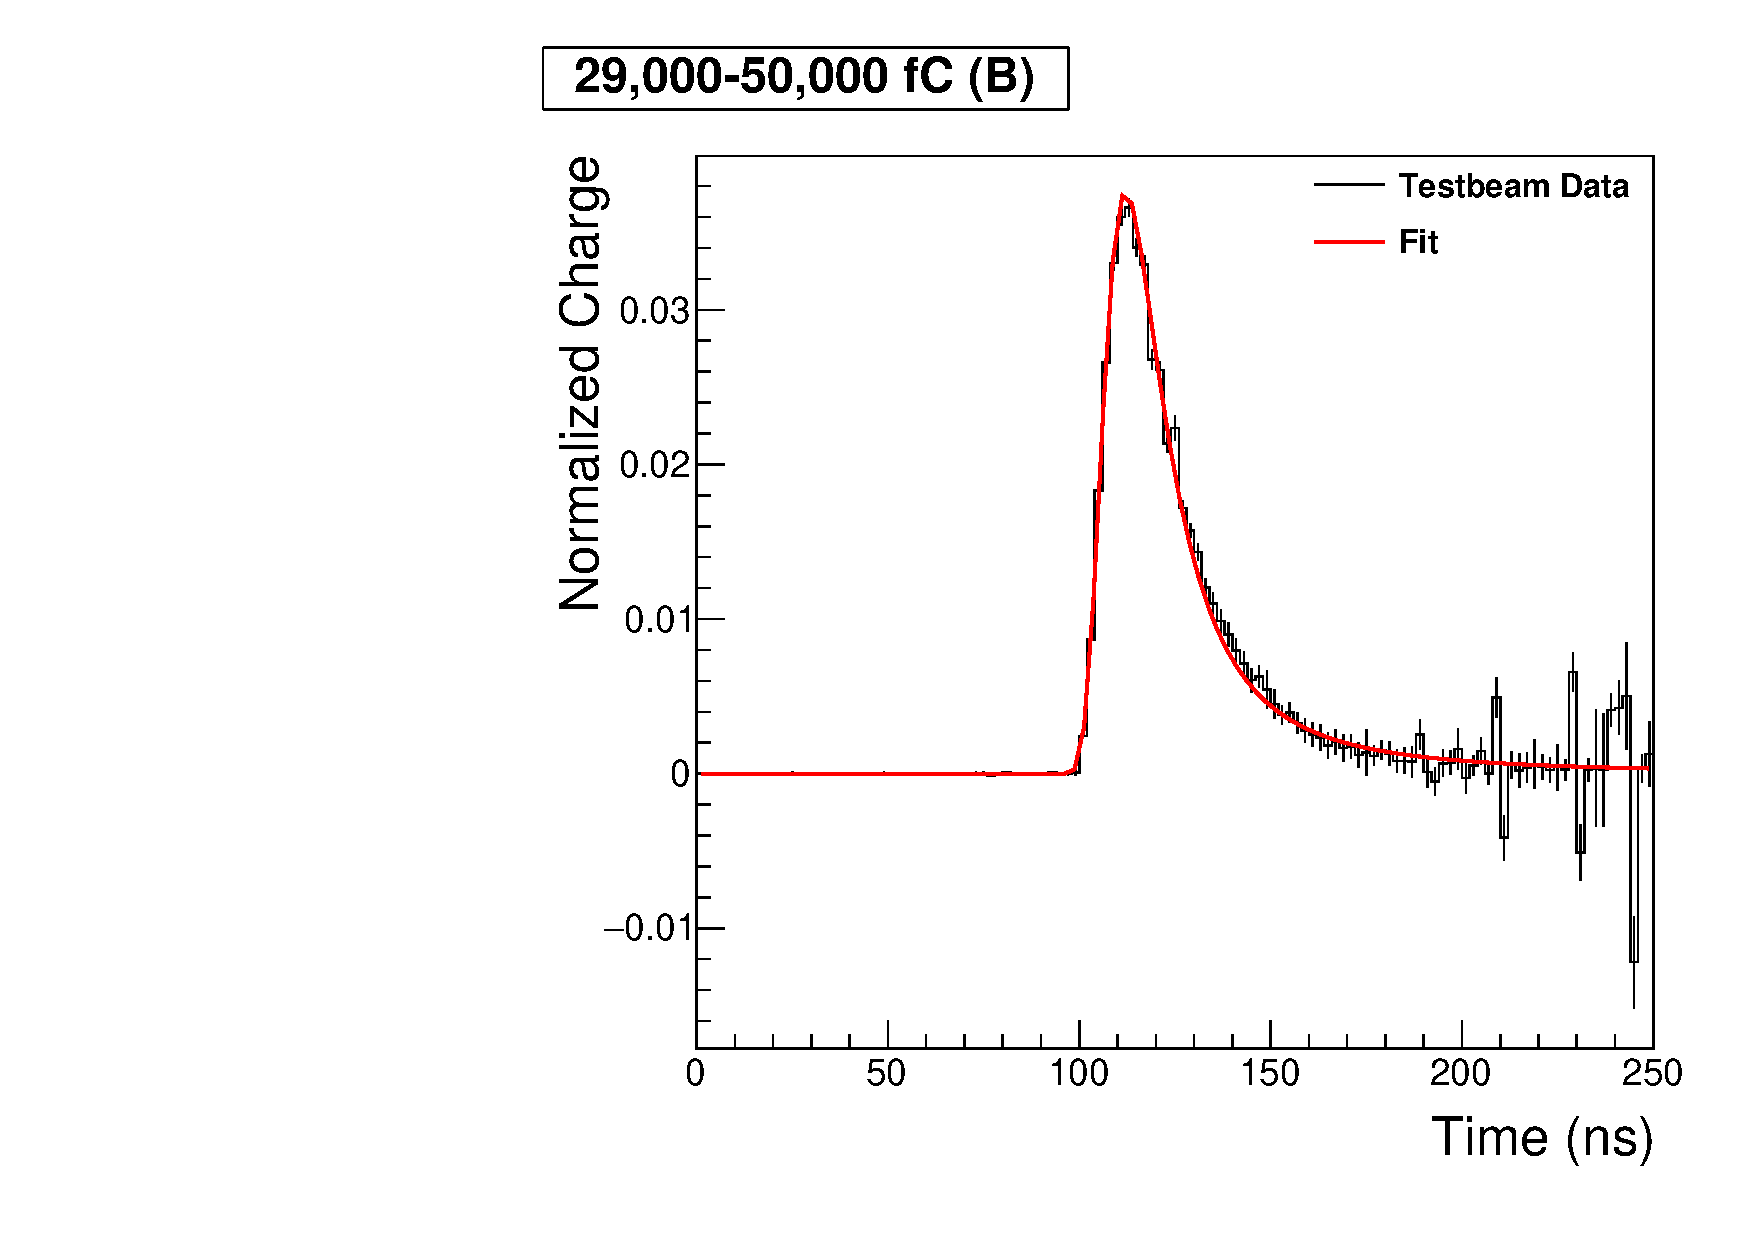
\includegraphics[width=0.495\linewidth]{Figures/29FittedPlot.pdf}
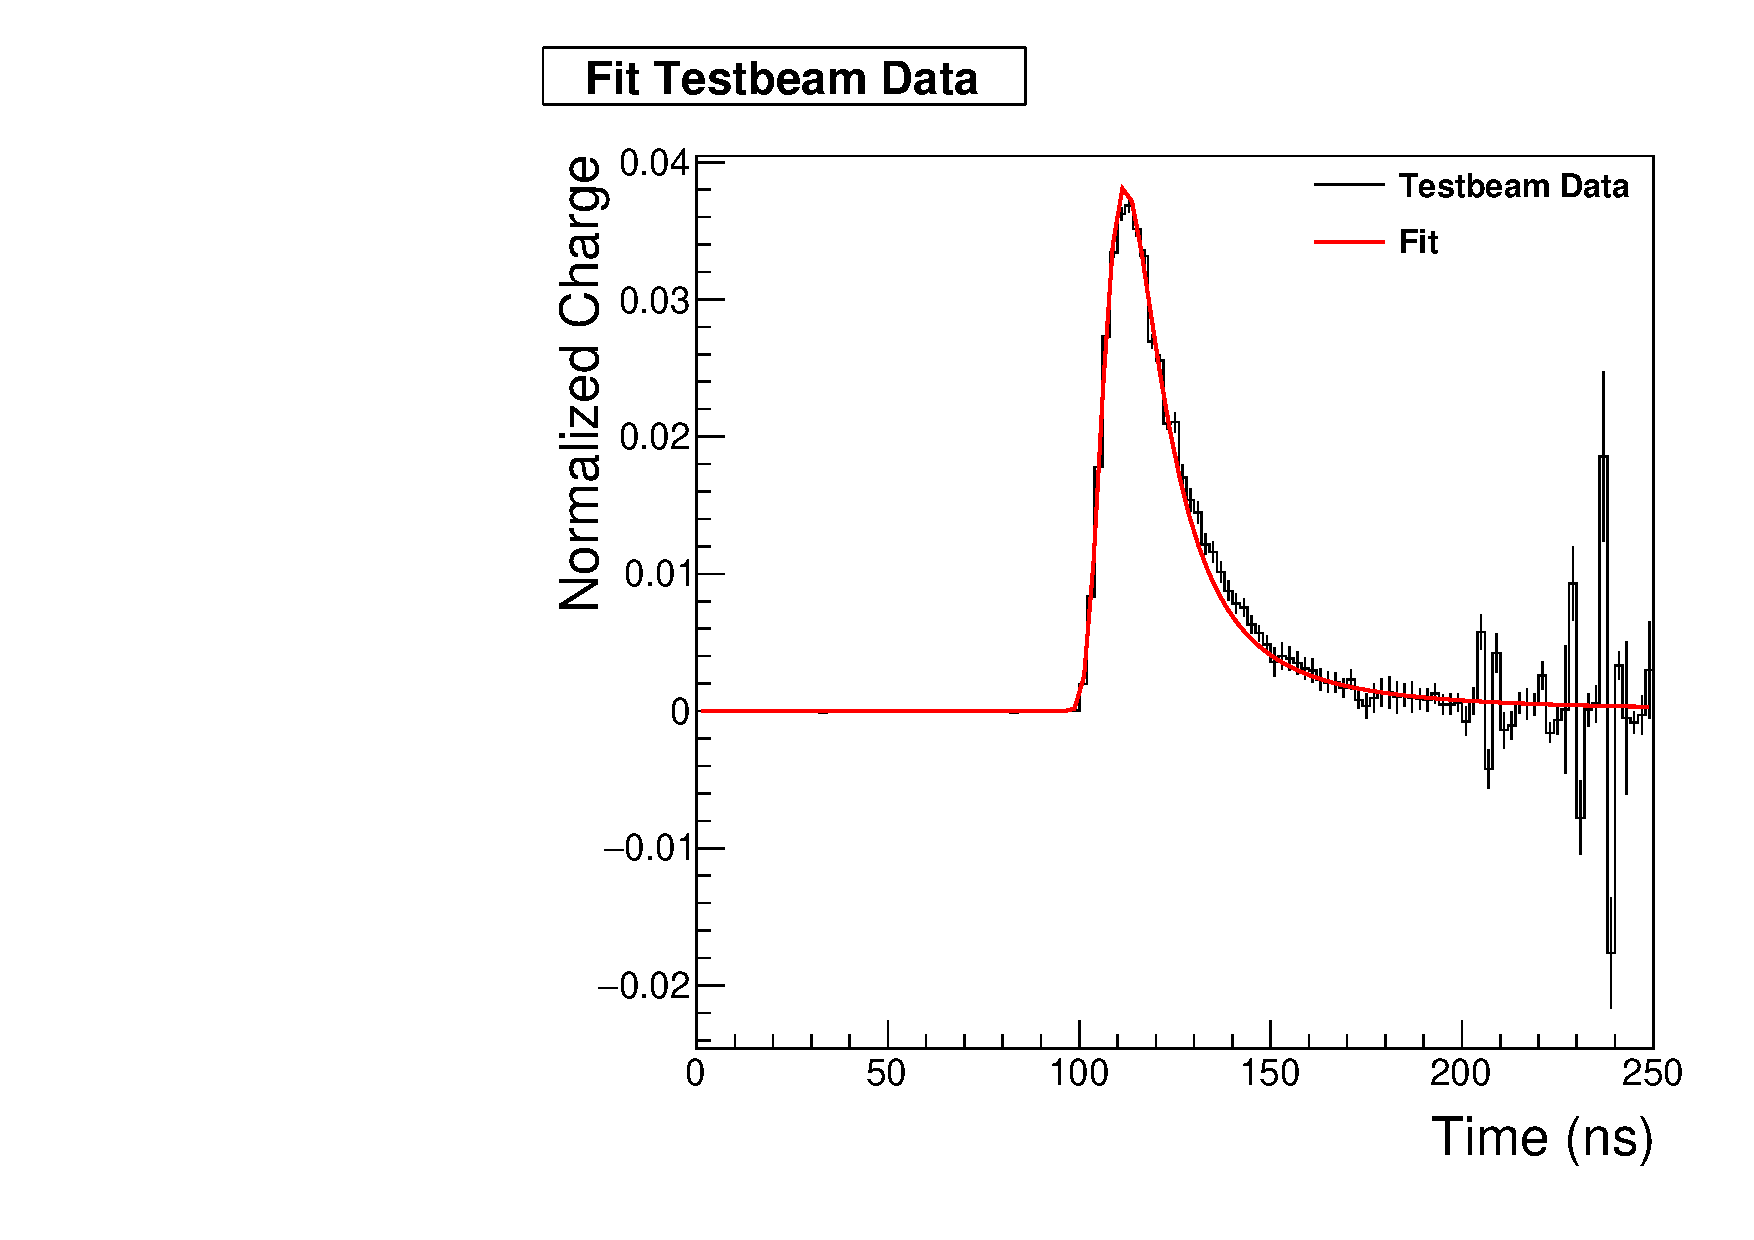
\includegraphics[width=0.495\linewidth]{Figures/50FittedPlot.pdf}
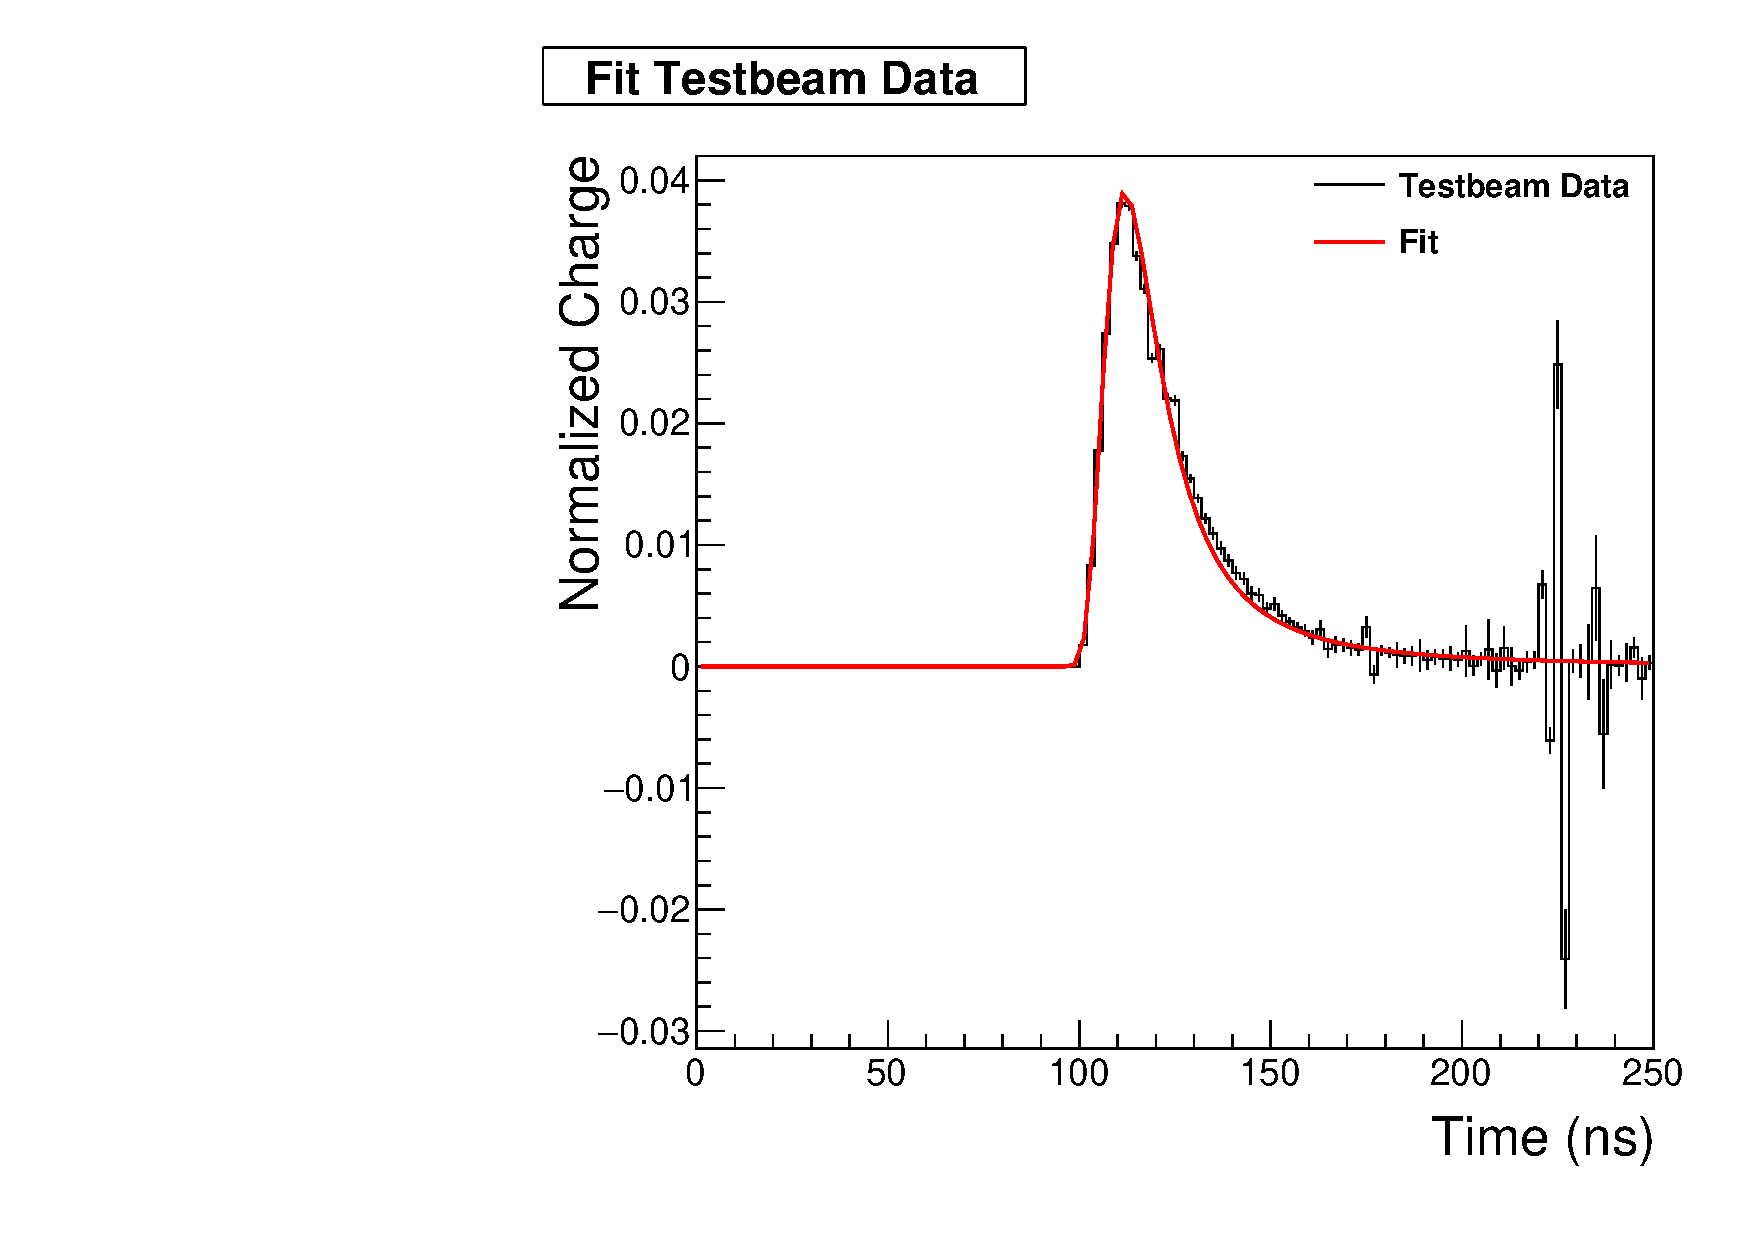
\includegraphics[width=0.495\linewidth]{Figures/80FittedPlot.pdf}
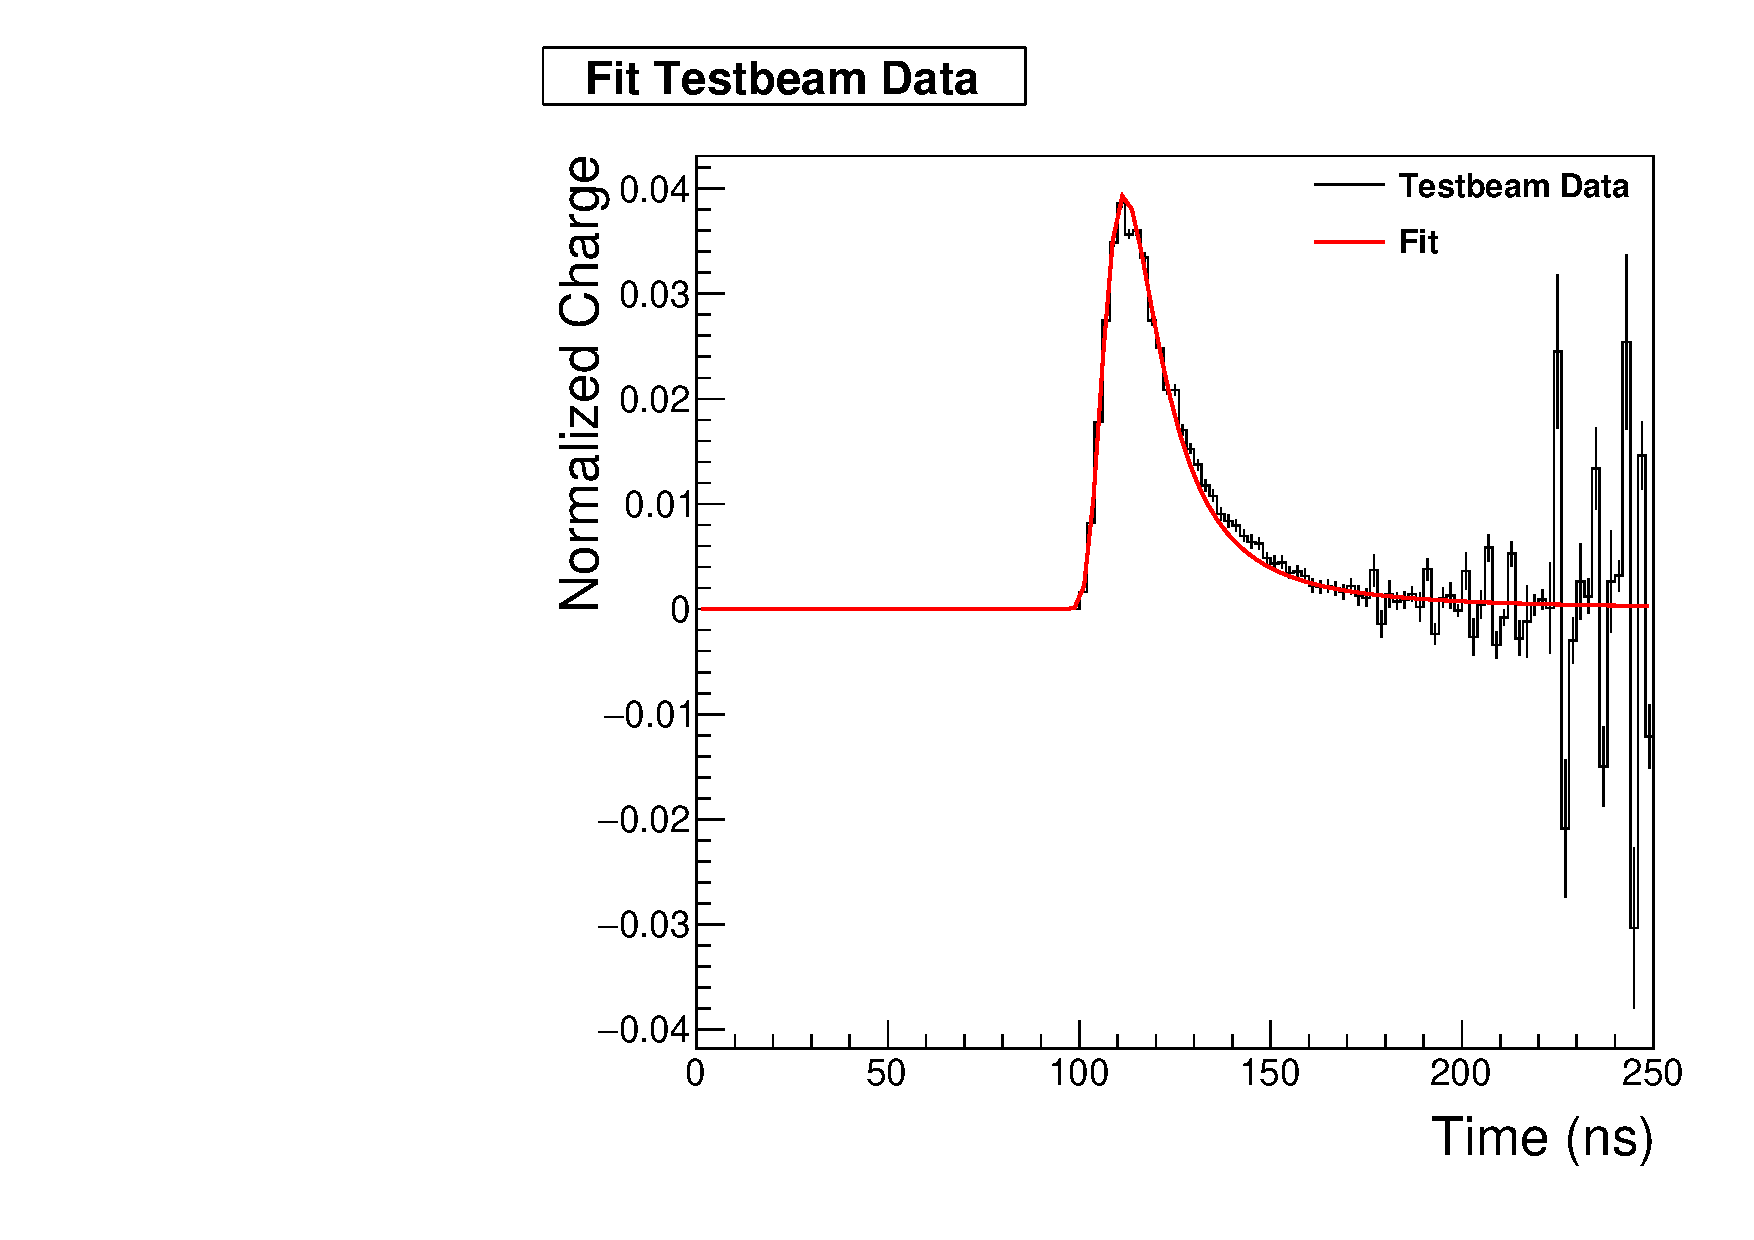
\includegraphics[width=0.495\linewidth]{Figures/125FittedPlot.pdf}
\caption{Fitted pulse shapes of using events of charge 10,000-29,000 fC (A) 29,000-50,000 fC (B) 50,000-80,000 fC (C) 80,000-125,000 fC (D) and 125,000-168,000 fC (E)}
\label{fig:fit_together}
\end{figure}

\begin{figure}
\centering
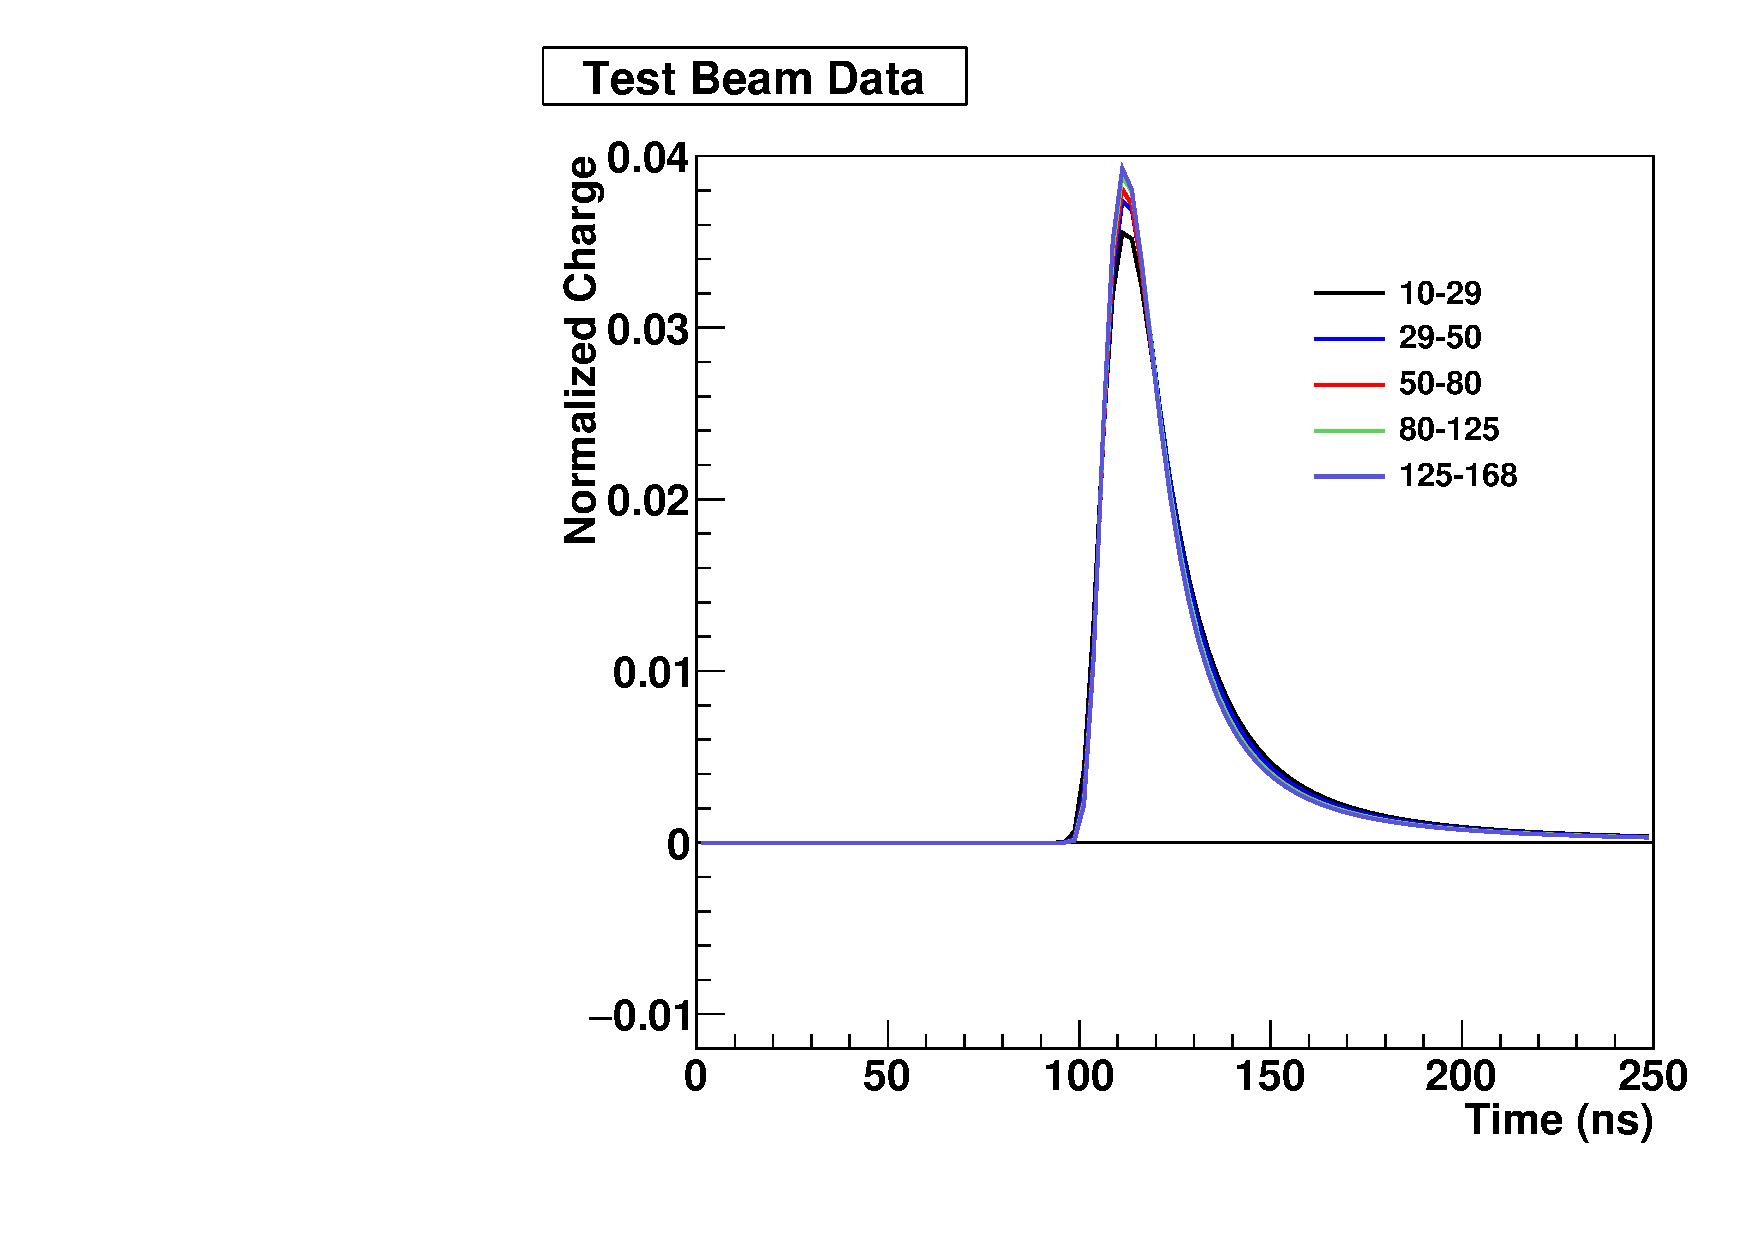
\includegraphics[width=0.8\linewidth]{Figures/Overlap.pdf}
\caption{The comparison of the fits to the pulse shapes obtained from the different charge ranges.}
\label{fig:Overlap}
\end{figure}


\section{Conclusions}

Using the test beam data we were able to extract a precise pulse shape of the new readout modules. This pulse shape does appear close to expectations and have a reasonable fit to the Landau Gaussian function. The pulse shape does show minor changes with changes in the output charge but at the energies from the test beam there was very little changes. The non-linearity of the SiPM was not able to be studied in depth using the test beam data, but we were able to confirm that at energies from the test beam the SiPMs are very close to linear. These readout modules were installed in the HE on the CMS detector over the winter of 2018. 

